\documentclass[journal]{IEEEtran}
% Overleaf: New Project > Upload Project (zip of this folder). Compiler: pdfLaTeX. Main document: main.tex.
\usepackage[utf8]{inputenc}
\usepackage[T1]{fontenc}
\usepackage{amsmath,amssymb,bm}
\usepackage{graphicx}
\usepackage{booktabs,multirow,array}
\usepackage[caption=false,font=footnotesize]{subfig}
\usepackage{siunitx}
\sisetup{per-mode=symbol,range-phrase=--,range-units=single}
\usepackage{xcolor}
\usepackage{tikz}
\usetikzlibrary{arrows.meta,positioning,shapes.geometric,calc}
\usepackage{url}
\usepackage[hidelinks]{hyperref}
\usepackage{cleveref}
\usepackage{placeins}
\renewcommand{\topfraction}{0.9}\renewcommand{\dbltopfraction}{0.9}
\renewcommand{\textfraction}{0.07}\renewcommand{\floatpagefraction}{0.8}\renewcommand{\dblfloatpagefraction}{0.8}
\setcounter{topnumber}{3}\setcounter{dbltopnumber}{3}\setcounter{totalnumber}{5}
\graphicspath{{fig/}}
\newcommand{\Nm}{\si{\newton\metre}}

\begin{document}

\title{A Periodic-Sector 3-D Nonlinear Magnetostatic\\ FEA Tool for Axial-Flux Machines:\\ Verification, Benchmarking and Application to the\\ TREN-V4 Halbach Actuator Motor}

\author{Qihao,~\IEEEmembership{osstrich Block2 Actuator Project}%
\thanks{Report date: 15 October 2026, revised 16 October 2026 (magnet grade selection). The solver is available as openFLUX, see the Appendix. Numerical work and drafting were assisted by Claude (Anthropic).}}

\markboth{osstrich Block2 Actuator Project --- Technical Report TREN-V4-M-03, October~2026}%
{Periodic-Sector 3-D FEA of the TREN-V4 Axial-Flux Motor}

\maketitle

\begin{abstract}
The TREN-V4 legged-robot actuator uses a single-sided, 27-slot/30-pole axial-flux permanent-magnet motor with a Hiperco~50 tape-wound stator and a Halbach rotor on a non-magnetic carrier. Because tooth width, pole arc and slot pitch all vary with radius, and because the active annulus is only \SI{12}{mm} wide against a \SI{0.4}{mm} air gap, a two-dimensional or multi-slice model cannot capture the end-region leakage that limits torque at high current. This report documents an open-source, full three-dimensional nonlinear magnetostatic finite-element tool written for this machine on top of NGSolve/Netgen. It uses a magnetic vector potential formulation with N\'ed\'elec edge elements, an energy-based Newton solver with line search, a BDDC-preconditioned conjugate-gradient linear solver, rotational periodicity over one third of the machine, and Arkkio's volume-averaged Maxwell stress for torque. Discretisation error is below \SI{1}{\percent}. Against the authors' own multi-slice 2-D model the full 3-D model predicts \SIrange{7}{10}{\percent} less torque at 200--\SI{250}{A}. Rebuilt on a published 45-slot/10-pole axial-flux prototype, the method reproduces the measured saturation slope and over-predicts measured shaft torque by a nearly constant \SIrange{5.6}{6.7}{\percent} at loaded operating points. For the TREN-V4 v4b rotor the tool predicts \SI{41.5}{\Nm} at \SI{250}{A} peak with ideal materials. Combining the benchmark error with 3-D sensitivity runs on stacking factor, magnet remanence, air gap, magnet joints and core quality, the realistic expectation for the built motor is about \SI{35}{\Nm} (range 33--\SI{38}{\Nm}). Finally, a surrogate of the 3-D field fitted to ten solves, validated to within \SI{0.7}{\percent}, is used with Monte Carlo tolerance analysis to choose magnet grades for the Halbach rotor on a 40Cr back ring. A rotor node added to the thermal model shows that the rotor stays below \SI{105}{\celsius} in sprint use and reaches about \SI{140}{\celsius} only in continuous running at the stator limit. SH and UH grades are limited to 41--\SI{108}{\celsius} at \SI{250}{A} by the reverse field in the side pieces. N48EH axial pieces with N45AH side pieces hold \SI{250}{A} up to \SI{145}{\celsius} and give \SI{42.5}{\Nm} cold with ideal materials.
\end{abstract}

\begin{IEEEkeywords}
Axial-flux permanent-magnet machine, finite-element analysis, edge elements, Halbach array, legged robot actuator, model validation, NGSolve.
\end{IEEEkeywords}

\section{Introduction}
\IEEEPARstart{A}{xial}-flux permanent-magnet (AFPM) machines give high torque per unit volume in short, large-diameter packages, which suits the joint actuators of dynamic legged robots \cite{gieras2008,aydin2004}. The TREN-V4 actuator replaces the TREN3 radial inrunner with a single-sided AFPM motor that sits around a \SI{80}{mm} gearbox bore. Its target is roughly \SI{35}{\Nm} of motor torque at \SI{250}{A} for short dashes, giving more than \SI{180}{\Nm} at the output through a 6.6:1 reduction.

AFPM geometry is inherently three-dimensional. The usual design practice is the \emph{quasi-3-D} or multi-slice method \cite{parviainen2005,gieras2008}. The annulus is cut into a few cylindrical slices, each slice is unrolled into a 2-D linear-machine model, and the slice results are summed. This captures radial variation of pole arc and tooth width but neglects three effects: flux fringing at the inner and outer radii, end-turn fields, and the radial flux component that couples neighbouring slices. In a machine whose active radial length (\SI{12}{mm}) is only about 30 times its air gap, and whose teeth saturate at peak current, these effects are not small. Published AFPM studies therefore increasingly use full 3-D FEA, typically presented as a periodic-sector mesh, $|B|$ shading on stator and rotor surfaces, air-gap flux-density distributions at the mean radius, and torque/back-EMF curves \cite{inwheel2021,magshape2018,wind2017,bench2122}.

This report presents a full-3-D nonlinear magnetostatic tool written for TREN-V4, in the same physical formulation as commercial packages such as Ansys Maxwell~3D, and uses it to answer one practical question: \emph{how much of the predicted \SI{41.5}{\Nm} will the built motor deliver?} The contributions are:
\begin{enumerate}
\item a documented, scriptable, open-source 3-D AFPM solver (\cref{sec:method}) and its comparison with established programs (\cref{sec:compare});
\item verification by mesh refinement and against the authors' multi-slice 2-D model, and validation by rebuilding a published, measured AFPM prototype (\cref{sec:verify});
\item a complete 3-D field and performance analysis of the TREN-V4 motor with the v4b Halbach rotor, shown both as 3-D renders and as 2-D slices of the 3-D solution (\cref{sec:results});
\item a quantified estimate of the torque the built motor will produce (\cref{sec:realistic}).
\end{enumerate}

\section{Machine Under Study}\label{sec:machine}
\Cref{tab:spec} lists the motor; \cref{fig:exploded} shows the 3-D model. The stator is a Hiperco~50 tape-wound core (\SI{0.1}{mm} tape) with 27 open, parallel-sided slots and pre-formed edgewise coils of 9 turns. The v4b rotor is a 60/40 Halbach array: 30 axially magnetised pieces spanning \SI{60}{\percent} of the pole pitch and 30 tangentially magnetised pieces filling the rest, \SI{5}{mm} thick, bonded to a 7075 aluminium carrier with no back iron \cite{halbach1980}. The 27/30 combination has $\gcd(27,30)=3$, so one third of the machine (9 slots, 10 poles) is the smallest periodic unit, and the cogging period is \SI{1.33}{\degree} mechanical (LCM 270).

\begin{table}[!t]
\caption{TREN-V4 motor with the v4b Halbach rotor (as modelled)}\label{tab:spec}
\centering\footnotesize
\begin{tabular}{@{}l>{\raggedright\arraybackslash}p{52mm}@{}}
\toprule
Topology & single-sided AFPM, slotted stator, Halbach rotor\\
Slots / poles & 27 / 30 (15 pole pairs), concentrated, double layer\\
Magnet annulus $R_i$ / $R_o$ & \SI{44.5}{mm} / \SI{56.5}{mm}\\
Stator yoke / tooth height & \SI{3.0}{mm} / \SI{8.6}{mm}, slot width \SI{6.0}{mm}\\
Air gap & \SI{0.4}{mm}\\
Rotor & 60/40 Halbach, \SI{5}{mm} NdFeB, 7075 carrier\\
Magnet model & $B_r=\SI{1.40}{T}$ (\SI{20}{\celsius}), $\mu_r=1.05$, linear\\
Core material & Hiperco 50 (Fe-49Co-2V), nonlinear $B$--$H$\\
Winding & 9 turns/coil, 1 path, star; $R_\mathrm{ph}=\SI{31}{m\ohm}$ at \SI{20}{\celsius}\\
Peak current & \SI{250}{A} (phase, peak)\\
\bottomrule
\end{tabular}
\end{table}

\begin{figure}[!t]
\centering
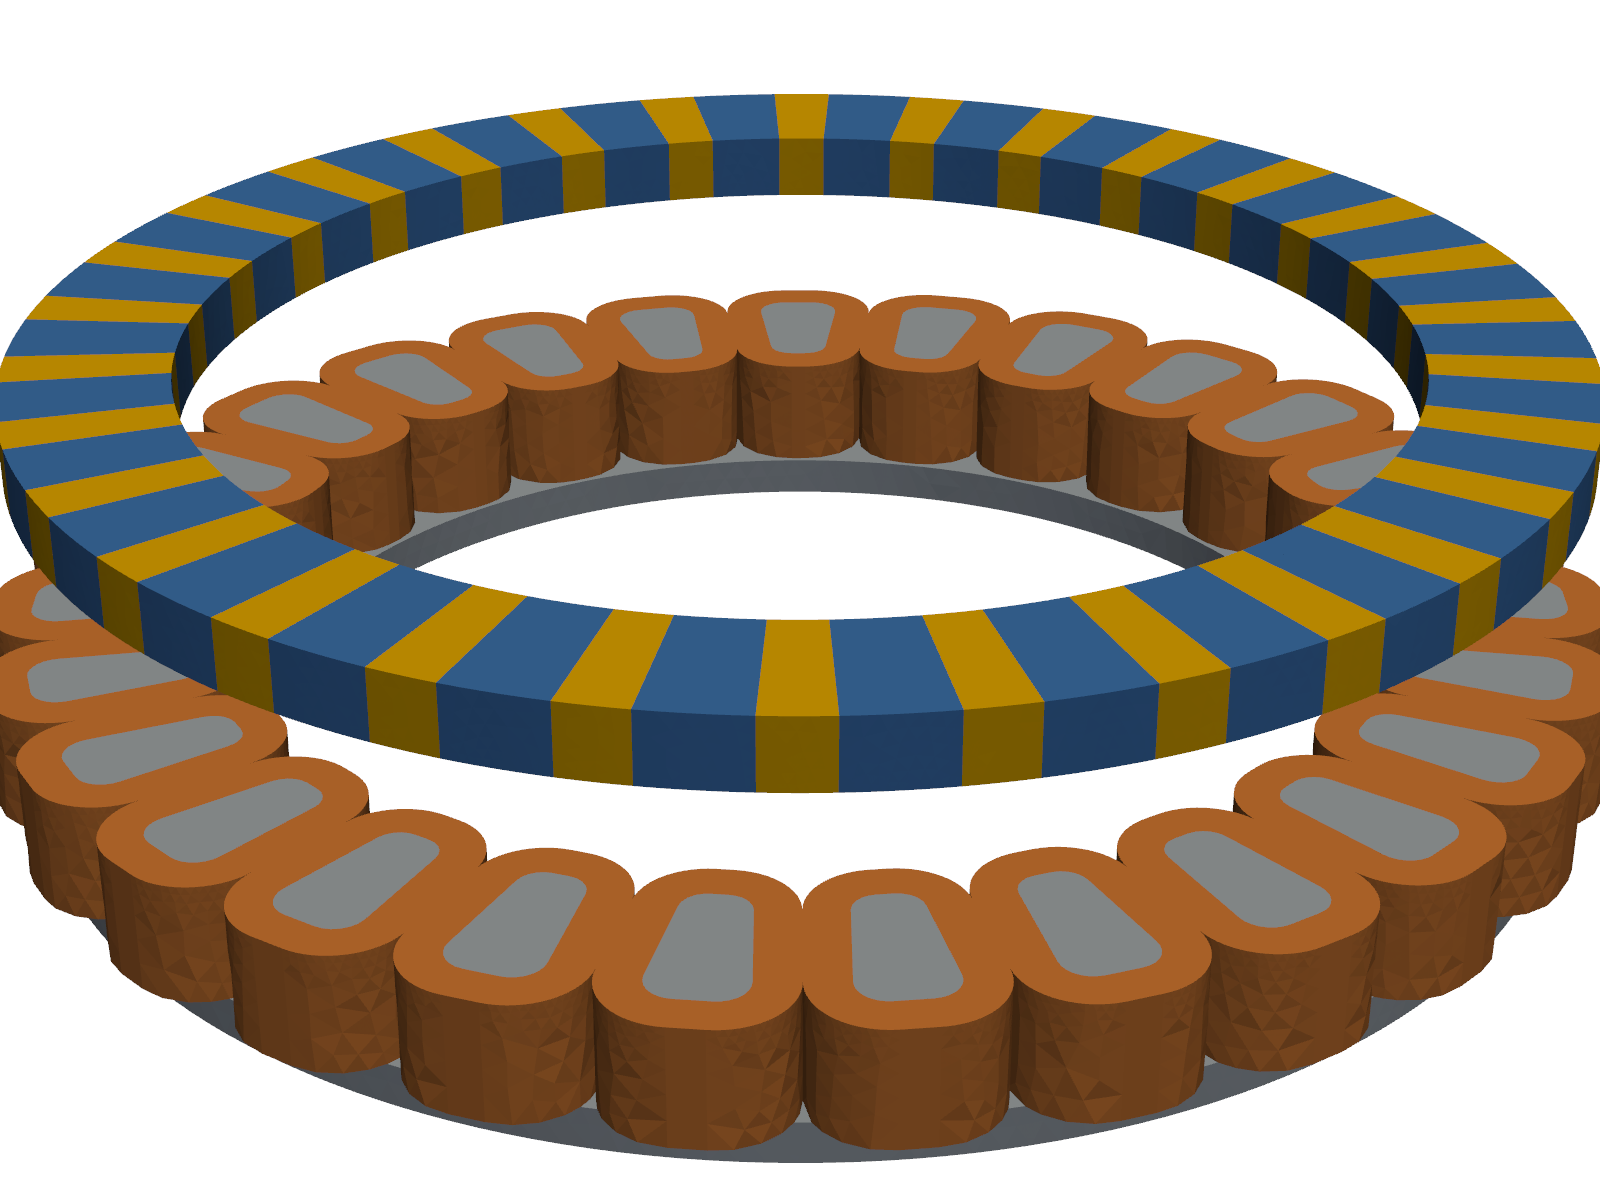
\includegraphics[width=\columnwidth,trim=0 60 0 40,clip]{r3d_exploded.png}
\caption{3-D model of the TREN-V4 motor (three periodic sectors), with the rotor lifted by \SI{14}{mm} to expose the stator. Grey: Hiperco~50 core; copper: tooth coils; blue: axially magnetised pieces; yellow: tangentially magnetised Halbach pieces.}
\label{fig:exploded}
\end{figure}

\section{Numerical Method}\label{sec:method}

\subsection{Formulation}
With no eddy currents, the field satisfies $\nabla\times\bm{H}=\bm{J}_s$ and $\nabla\cdot\bm{B}=0$. Writing $\bm{B}=\nabla\times\bm{A}$, the solution minimises the energy functional
\begin{multline}
\Pi(\bm{A})=\int_\Omega W\!\left(|\nabla\times\bm{A}|\right)\mathrm{d}V\\
-\int_{\Omega_m}\nu_m B_r\,\hat{\bm{m}}\cdot(\nabla\times\bm{A})\,\mathrm{d}V-\int_{\Omega_c}\bm{J}_s\cdot\bm{A}\,\mathrm{d}V,
\label{eq:energy}
\end{multline}
where $W(B)=\int_0^B H(b)\,\mathrm{d}b$ is the magnetic energy density, $\hat{\bm{m}}$ the magnetisation direction and $\nu_m=1/(\mu_0\mu_r)$. In air and coils $W=B^2/(2\mu_0)$; in magnets $W=\nu_m B^2/2$; in the core $W$ is obtained by integrating a piecewise-linear $H(B)$ spline built from the Hiperco~50 curve and extended with slope $1/\mu_0$ above \SI{2.6}{T}, which makes $W$ convex and $C^1$.

$\bm{A}$ is discretised with first-order (and, for verification, second-order) N\'ed\'elec edge elements $H(\mathrm{curl})$ \cite{nedelec1980} on a tetrahedral mesh, with gradient degrees of freedom removed. A tiny regularisation term $10^{-6}\nu_0|\bm{A}|^2/2$ fixes the gauge. The coil current density is projected onto the discretely divergence-free space by solving $\Delta\phi=\nabla\cdot\bm{J}_s$ and using $\bm{J}_s-\nabla\phi$, so the right-hand side is consistent with the kernel of the curl operator.

\subsection{Nonlinear and linear solvers}
\Cref{eq:energy} is minimised by Newton's method on the exact linearisation, with a backtracking line search that halves the step until the energy decreases. Convergence to a relative residual of $10^{-4}$ typically takes 10--14 iterations at \SI{250}{A}. Each linear step is solved by conjugate gradients preconditioned with balancing domain decomposition by constraints (BDDC) \cite{mandel1997}, as implemented in NGSolve \cite{schoberl2014}.

\subsection{Geometry, periodicity and mesh}
Geometry is generated parametrically with the OpenCASCADE kernel in Netgen \cite{schoberl1997}: stator yoke and trapezoidal teeth with rounded corners, coils as four straight bars and four corner sectors per tooth (each with its own current direction field), magnet pieces as annular sectors, and an air box from $r=32$ to \SI{70}{mm} extending \SI{6}{mm} beyond the stack axially. The sector boundaries lie on slot centre lines, so no tooth or coil is cut; magnets that cross a boundary are split. Faces on the two sector planes are identified with a \SI{120}{\degree} rotation, which enforces $\bm{A}(\mathcal{R}\bm{x})=\mathcal{R}\bm{A}(\bm{x})$ (even periodicity, since 10 poles complete five electrical periods). Local mesh sizes are \SI{0.5}{mm} in the gap, \SI{1.2}{mm} in magnets and \SI{1.8}{mm} in core and coils. \Cref{fig:mesh} shows the result: \num{292176} tetrahedra and \num{344397} unknowns.

\begin{figure}[!t]
\centering
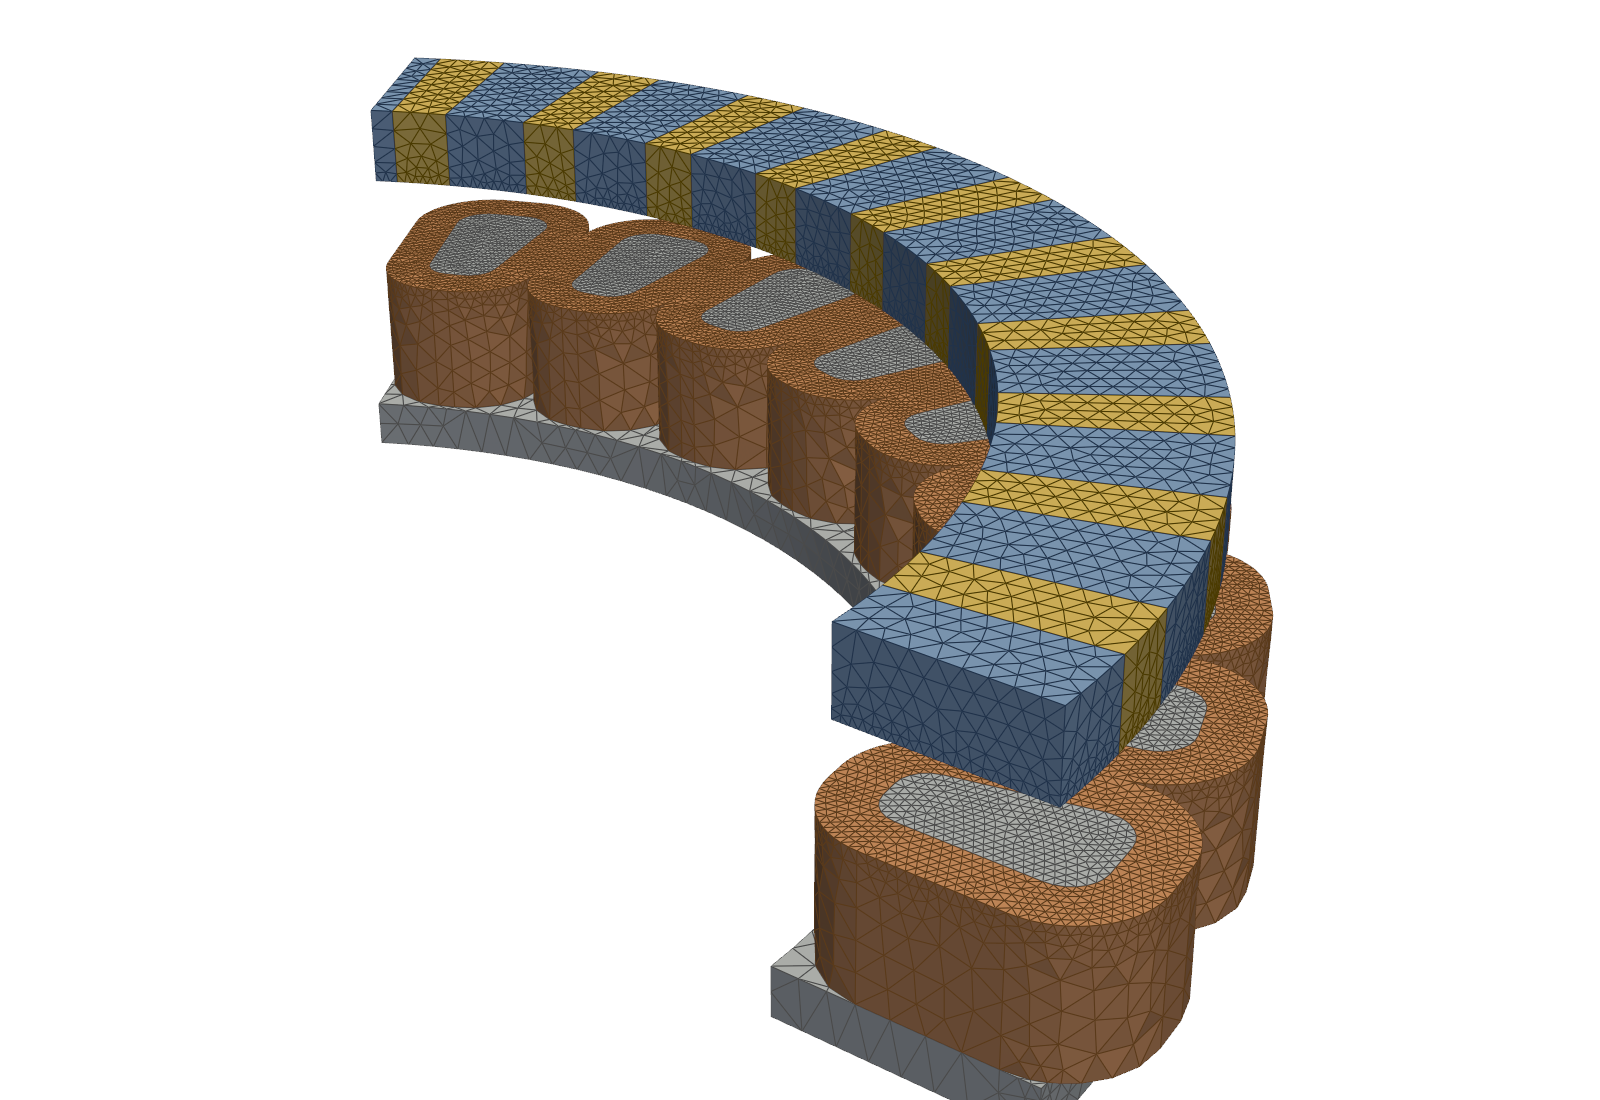
\includegraphics[width=\columnwidth,trim=300 0 250 40,clip]{r3d_mesh.png}
\caption{Computational domain (one 120\si{\degree} periodic sector, 9 slots and 10 poles) and surface mesh. The magnet layer is shown displaced upward by \SI{6}{mm}; air, gap and air-box elements are hidden.}
\label{fig:mesh}
\end{figure}

\subsection{Post-processing}
Electromagnetic torque uses Arkkio's method \cite{arkkio1987}, i.e.\ the Maxwell stress averaged over the whole gap volume $V_g$ of axial thickness $g$:
\begin{align}
T&=\frac{3}{g\,\mu_0}\int_{V_g} r\,B_\theta B_z\,\mathrm{d}V ,\\
F_z&=\frac{3}{g}\int_{V_g}\frac{B_z^2-B_r^2-B_\theta^2}{2\mu_0}\,\mathrm{d}V ,
\end{align}
where the factor 3 restores the full machine. Volume averaging makes the result far less sensitive to the gap mesh than a single-surface stress integral. Phase flux linkage is $\psi=N/S_c\int_{\Omega_c}\hat{\bm{t}}\cdot\bm{A}\,\mathrm{d}V$ summed over the coils of each phase. Demagnetisation risk is assessed from the opposing field $H_{op}=(B_r-\hat{\bm{m}}\cdot\bm{B})/(\mu_0\mu_r)$ sampled at \num{300000} random points in the magnets.

\begin{figure}[!t]
\centering\footnotesize
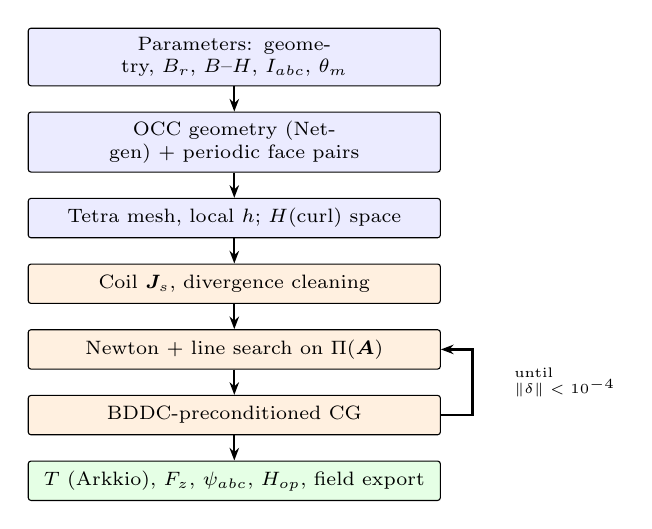
\begin{tikzpicture}[node distance=3.2mm,
  box/.style={draw,rounded corners=1pt,align=center,minimum width=52mm,text width=50mm,minimum height=5mm,font=\scriptsize,fill=#1},box/.default=white,
  arr/.style={-{Stealth[length=1.6mm]},thick}]
\node[box=blue!8] (p) {Parameters: geometry, $B_r$, $B$--$H$, $I_{abc}$, $\theta_m$};
\node[box=blue!8,below=of p] (g) {OCC geometry (Netgen) + periodic face pairs};
\node[box=blue!8,below=of g] (m) {Tetra mesh, local $h$; $H(\mathrm{curl})$ space};
\node[box=orange!12,below=of m] (j) {Coil $\bm{J}_s$, divergence cleaning};
\node[box=orange!12,below=of j] (n) {Newton + line search on $\Pi(\bm{A})$};
\node[box=orange!12,below=of n] (l) {BDDC-preconditioned CG};
\node[box=green!10,below=of l] (o) {$T$ (Arkkio), $F_z$, $\psi_{abc}$, $H_{op}$, field export};
\draw[arr] (p)--(g); \draw[arr] (g)--(m); \draw[arr] (m)--(j); \draw[arr] (j)--(n); \draw[arr] (n)--(l);
\draw[arr] (l.east) -- ++(4mm,0) |- (n.east) node[pos=0.25,right,font=\tiny,align=left,xshift=4mm]{until\\$\|\delta\|<10^{-4}$};
\draw[arr] (l)--(o);
\end{tikzpicture}
\caption{Solution flow of the 3-D tool. One rotor position and current set is one solve, about 15 minutes on one CPU core with \SI{6}{GB} of memory.}
\label{fig:flow}
\end{figure}

\section{Comparison With Existing Programs}\label{sec:compare}
\Cref{tab:programs} places the tool among programs commonly used for AFPM design. Physically it solves the same problem as the magnetostatic solvers of the commercial 3-D packages: an $\bm{A}$-formulation on edge elements with nonlinear materials. On identical geometry, mesh density and $B$--$H$ data, these should agree to within 1--\SI{2}{\percent}. What it lacks is motion with eddy currents (transient analysis), circuit coupling and a graphical pre-processor. What it adds is a fully parametric, scriptable model that runs anywhere Python runs, at no licence cost, and that can be modified for unusual features such as Halbach joints, partial back iron or stacking factor.

\begin{table*}[!t]
\caption{Present tool compared with established electromagnetic FEA programs for AFPM design (capabilities in general terms)}\label{tab:programs}
\centering\footnotesize
\setlength{\tabcolsep}{3pt}\scriptsize
\begin{tabular}{@{}>{\raggedright}p{27mm}>{\raggedright}p{30mm}>{\raggedright}p{20mm}>{\raggedright}p{36mm}>{\raggedright}p{26mm}>{\raggedright\arraybackslash}p{22mm}@{}}
\toprule
Program & Dimensionality / formulation & Nonlinear solver & AFPM-specific features & Transient / motion & Access \\
\midrule
\textbf{Present tool} (NGSolve) & Full 3-D, $\bm{A}$ on N\'ed\'elec edges, order 1--2 & Newton, energy line search & Parametric 120\si{\degree} periodic sector; Halbach, joints, stacking factor & No (magnetostatic, multi-position) & Open source, Python scripted\\
Ansys Maxwell 3D & Full 3-D, $\bm{A}$--$\phi$ / $T$--$\Omega$, adaptive mesh & Newton & Periodic/master--slave boundaries, motion band & Yes, with eddy currents & Commercial\\
JMAG-Designer & 2-D and 3-D, edge elements & Newton (ICCG) & AFPM templates, 3-D sliding mesh & Yes & Commercial\\
COMSOL AC/DC & 2-D and 3-D, $\bm{A}$ or mixed & Newton & General multiphysics, rotating machinery interface & Yes & Commercial\\
Altair Flux 3D / Simcenter MAGNET / Opera 3D & Full 3-D, edge or nodal + scalar potentials & Newton & Periodicity, motion & Yes & Commercial\\
Ansys Motor-CAD & 2-D FEA, AFPM via multi-slice & Newton & Fast templated AFPM design & Steady-state sweeps & Commercial\\
FEMM 4.2 \cite{femm} & 2-D planar/axisymmetric only & Newton & Single unrolled slice (as \texttt{femm\_slice.lua}) & No & Freeware, Windows\\
Own multi-slice 2-D (TREN-V4 v0.1--0.4) & 2-D, bilinear quads, 4 radial slices & Newton & Unrolled slices, periodic & No & In-house Python\\
\bottomrule
\end{tabular}
\end{table*}

The more important comparison for design decisions is with the multi-slice 2-D model that sized the motor (\cref{fig:quasi3d}). \Cref{fig:2d3d} compares both on the v0.4 design (\SI{0.7}{mm} gap, steel back iron). At low current the 3-D model gives only \SI{2}{\percent} less flux, the expected radial-fringing loss. The difference grows to \SI{7}{\percent} at \SI{200}{A} and \SI{10}{\percent} at \SI{250}{A}, because leakage flux around the ends of the teeth adds to tooth-root and yoke saturation, which 2-D slices cannot represent. A fixed ``2-D minus \SI{6}{\percent}'' allowance therefore overstates high-current torque. This is the main reason a full 3-D tool was built.

\begin{figure*}[!t]
\centering
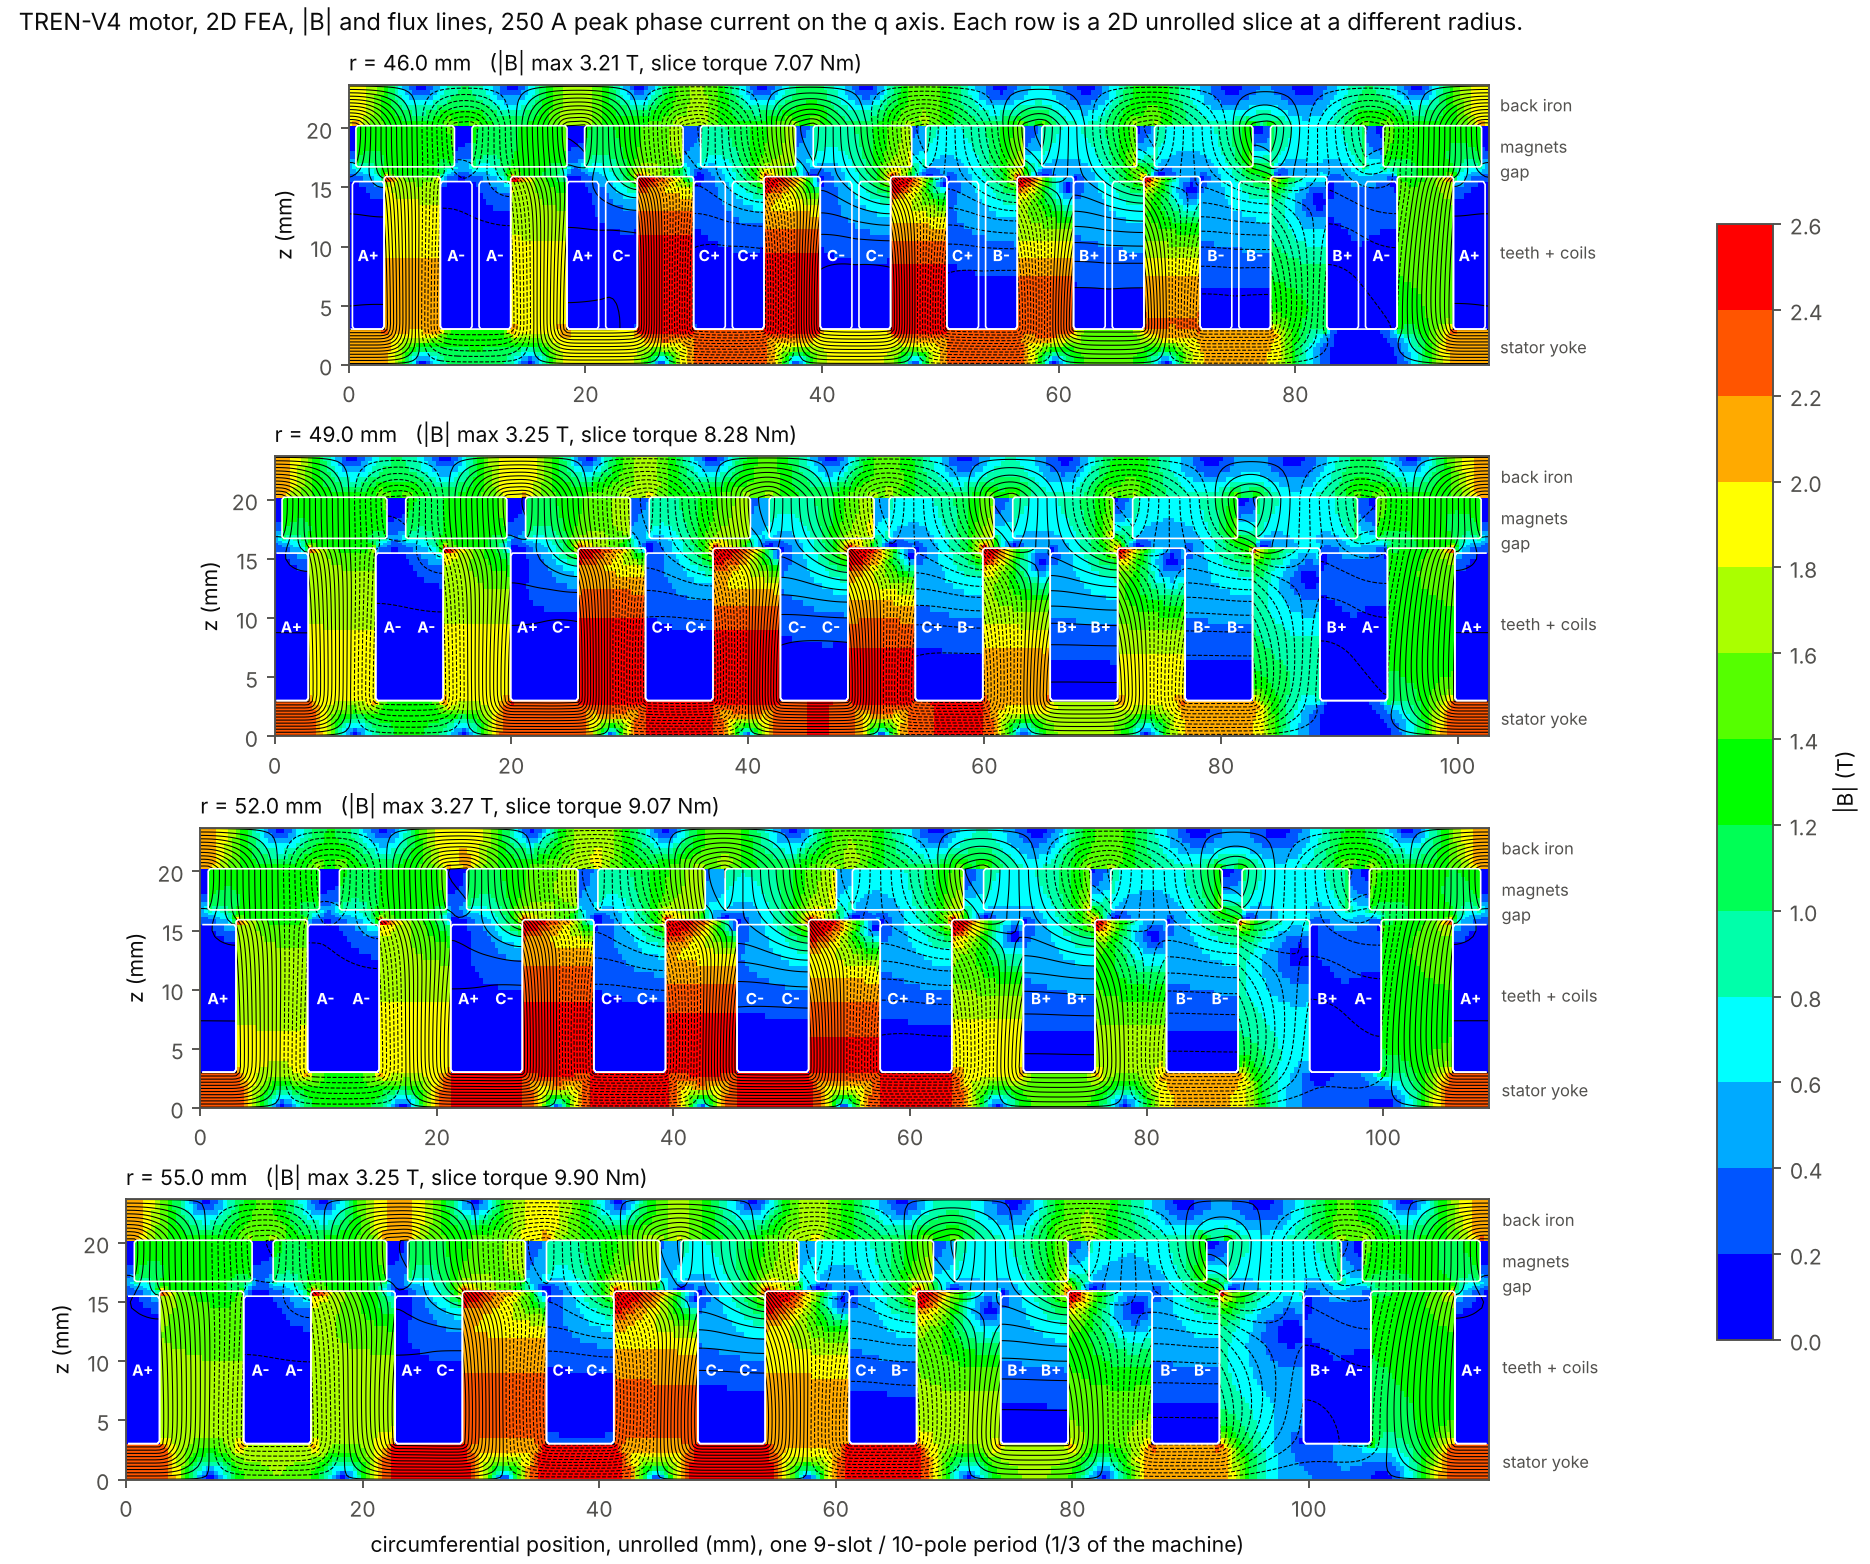
\includegraphics[width=0.86\textwidth]{quasi3d_v02.png}
\caption{The multi-slice (quasi-3-D) 2-D model used for initial sizing: $|B|$ and flux lines in four unrolled slices at $r=46$, 49, 52 and \SI{55}{mm}, \SI{250}{A} on the $q$ axis. This figure is from the earlier v0.2 geometry (\SI{13}{mm} teeth, steel back iron) and illustrates the method only.}
\label{fig:quasi3d}
\end{figure*}

\begin{figure}[!t]
\centering
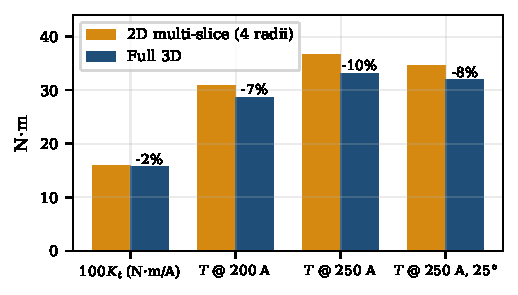
\includegraphics[width=\columnwidth]{2d_vs_3d.pdf}
\caption{Multi-slice 2-D model against full 3-D for the v0.4 design: low-current torque constant and torque at 200 and \SI{250}{A}. Labels give the 3-D change.}
\label{fig:2d3d}
\end{figure}

\section{Verification and Validation}\label{sec:verify}

\subsection{Discretisation}
\Cref{tab:conv} shows mesh and element-order refinement on the v0.4 design at \SI{200}{A}. Refining the gap mesh changes torque by \SI{0.35}{\percent}, and second-order elements by \SI{0.6}{\percent}. Varying rotor position across the ripple period (\num{0.5}, 1.0 and \SI{1.5}{\degree}) changes the v4b torque by $\pm\SI{0.3}{\percent}$ (\cref{fig:sens}). Discretisation and sampling error is therefore well below \SI{1}{\percent}, small compared with material and manufacturing uncertainty.

\begin{table}[!t]
\caption{Mesh convergence, v0.4 design, \SI{200}{A} $q$-axis}\label{tab:conv}
\centering\footnotesize
\begin{tabular}{@{}lrr@{}}
\toprule
Discretisation & Unknowns & Torque (\Nm)\\
\midrule
1st order, \SI{0.8}{mm} gap mesh & \num{143000} & 28.74\\
1st order, \SI{0.5}{mm} gap mesh & \num{341000} & 28.84\\
2nd order, \SI{0.8}{mm} gap mesh & \num{629000} & 28.90\\
\bottomrule
\end{tabular}
\end{table}

\subsection{Benchmark: a published AFPM prototype}
Few publications give both complete geometry and measured torque against current. The most complete found is the 64-kW double-stator, single-rotor AFPM of \cite{bench2122}: 45 slots, 10 poles, strip-wound M330-35A cores, an ironless rotor with \SI{10}{mm} N33EH magnets spanning 120\si{\degree} electrical, \SI{1.125}{mm} gaps, active diameters \SI{245}{}/\SI{140}{mm}, slots \SI{7}{}$\times$\SI{20}{mm} and \SI{8.5}{mm} yokes. Measured torque constant at seven currents, the authors' own 3-D FEA, and a measured line-to-line voltage constant of \SI{0.62}{V\,s/rad} are reported.

The machine was rebuilt with the same solver code, generalised to arbitrary slot/pole numbers (\texttt{geo\_af.py}, \texttt{solve\_af.py}). Only one stator is modelled, with a natural (flux-normal) boundary at the rotor mid-plane, over a 1/5 periodic sector (9 slots, 2 poles; \num{241666} tetrahedra). The $q=1.5$ double-layer winding is represented exactly in slot ampere-turns by equivalent tooth coils. Results are averaged over two rotor positions with the no-load cogging torque removed. Turns per coil and parallel paths are not published, so their ratio was set from the measured back-EMF. This gives 3.95, within \SI{1.3}{\percent} of the integer 4, which shows that the no-load flux of the model is consistent with the prototype. The comparison therefore tests the loaded behaviour.

\begin{figure*}[!t]
\centering
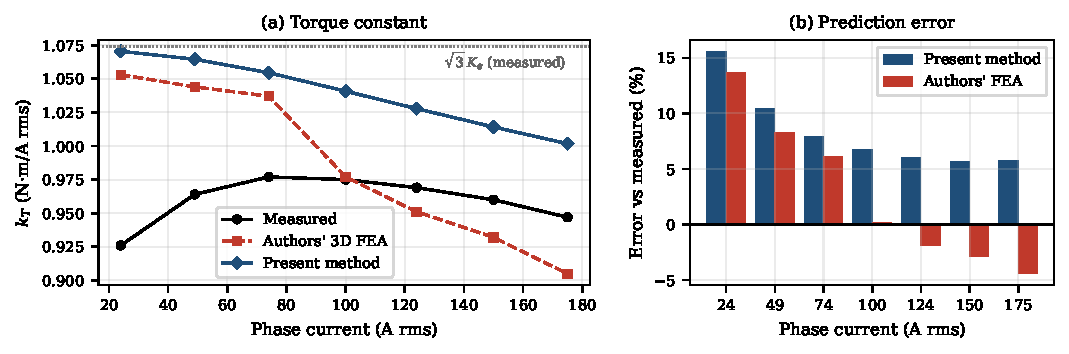
\includegraphics[width=\textwidth]{bench_kT.pdf}
\caption{Benchmark against the measured AFPM prototype of \cite{bench2122}. (a) Torque constant against phase current; (b) error relative to measurement. The present method is anchored to the measured back-EMF ($\sqrt3 K_e$, dotted).}
\label{fig:bench}
\end{figure*}

\Cref{fig:bench} shows the result. Between 100 and \SI{175}{A} the present method over-predicts measured torque by a nearly constant 5.6--\SI{6.7}{\percent}, and its fall in $k_T$ ($-\SI{3.7}{\percent}$) closely matches the measured fall ($-\SI{2.9}{\percent}$). The authors' 3-D FEA falls by \SI{7.4}{\percent} and agrees with measurement only near \SI{100}{A}, where its errors change sign. The larger discrepancy at low current is consistent with about \SI{1}{\Nm} of bearing, seal and iron-loss drag in the \SI{500}{rpm} shaft measurement. The remaining offset of about \SI{5}{\percent} is torque the prototype does not deliver even though its back-EMF says it should: thermal state during the test, rotor--stator misalignment (estimated by the authors at 1.6--\SI{5.6}{\percent}) and current-angle error.

\Cref{tab:lit} collects other published comparisons. The common pattern is that well-executed 3-D FEA reproduces no-load flux to within 1--\SI{5}{\percent}, while measured loaded torque lands 3--\SI{9}{\percent} \emph{below} the prediction. None of these sources reports measured torque above the FEA.

\begin{table}[!t]
\caption{Published 3-D FEA vs measurement on AFPM and related machines}\label{tab:lit}
\centering\footnotesize
\begin{tabular}{@{}>{\raggedright}p{32mm}>{\raggedright\arraybackslash}p{45mm}@{}}
\toprule
Machine & Reported FEA vs measured\\
\midrule
DSSR AFPM, 45/10 \cite{bench2122} & $K_e$ $-0.6$\,\%; $k_T$ $+0.2$ to $-4.4$\,\% (100--175 A), $+6$ to $+14$\,\% (low $I$)\\
DSSR AFPM, 18/12 \cite{stet2026} & torque within 3.5\,\% (20--400 A); $+75$\,\si{\celsius} on magnets: $-7$\,\% torque\\
YASA, SMC teeth \cite{yasa2025} & static torque 8.6\,\% off; back-EMF up to 20\,\% (EDM damage)\\
PCB-stator AFPM, micro-robot \cite{pcb2025} & back-EMF 5\,\% below simulation\\
SPM, 3-segment Halbach \cite{wevj2025} & back-EMF within 1.1\,\%\\
Prius 2004 IPM (radial) \cite{ornl2005} & \SI{400}{\Nm} needs \SI{250}{A}; saturation grows above \SI{250}{A}\\
\bottomrule
\end{tabular}
\end{table}

\section{3-D Results for TREN-V4}\label{sec:results}
All results in this section are for the v4b rotor at a rotor position of \SI{1.0}{\degree} mechanical. The current is on the $q$ axis unless stated, and materials are ideal: no stacking factor, \SI{20}{\celsius} magnets, no joints between pieces.

\subsection{Flux density in three dimensions}
\Cref{fig:statorB} shows $|B|$ on the stator surfaces at no load and at \SI{250}{A}, and \cref{fig:stats}(a) gives the volume distribution in the core. At no load only \SI{4}{\percent} of the core volume exceeds \SI{1.8}{T}. At \SI{250}{A}, \SI{51}{\percent} exceeds \SI{2.0}{T} and \SI{17}{\percent} exceeds \SI{2.35}{T}, the knee of Hiperco~50. The teeth that carry the summed magnet and armature flux are saturated over their full height. The saturation is strongest at the tooth tips facing the gap and at the inner and outer tooth ends, where end leakage adds to the main flux. This is the mechanism behind the 3-D torque deficit of \cref{fig:2d3d}. \Cref{fig:clip} cuts the model along a tooth centre plane, and \cref{fig:vectors} shows the direction of $\bm{B}$ in the core. Because first-order edge elements give a piecewise-constant $\bm{B}$, the surface maps show element-scale facets. These do not affect the integrated quantities (\cref{tab:conv}).

\begin{figure}[!t]
\centering
\subfloat[No load]{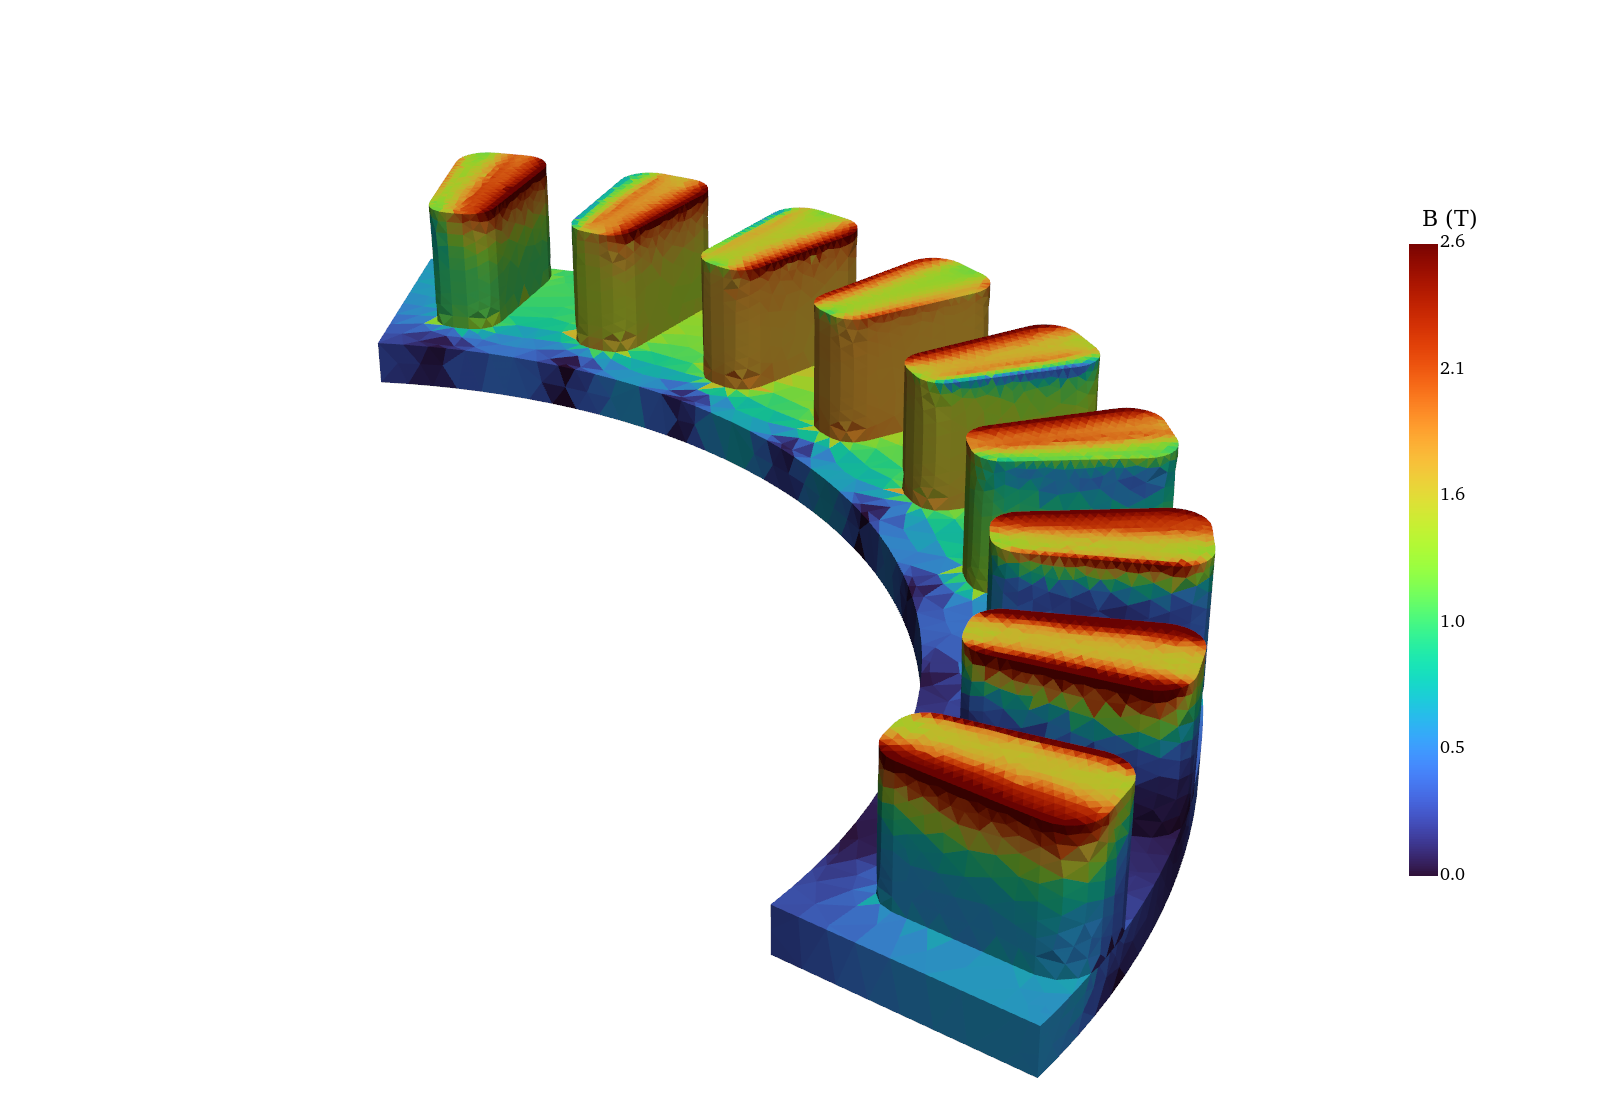
\includegraphics[width=0.49\columnwidth,trim=330 60 0 120,clip]{r3d_statorB_i0.png}}\hfil
\subfloat[\SI{250}{A}, $q$ axis]{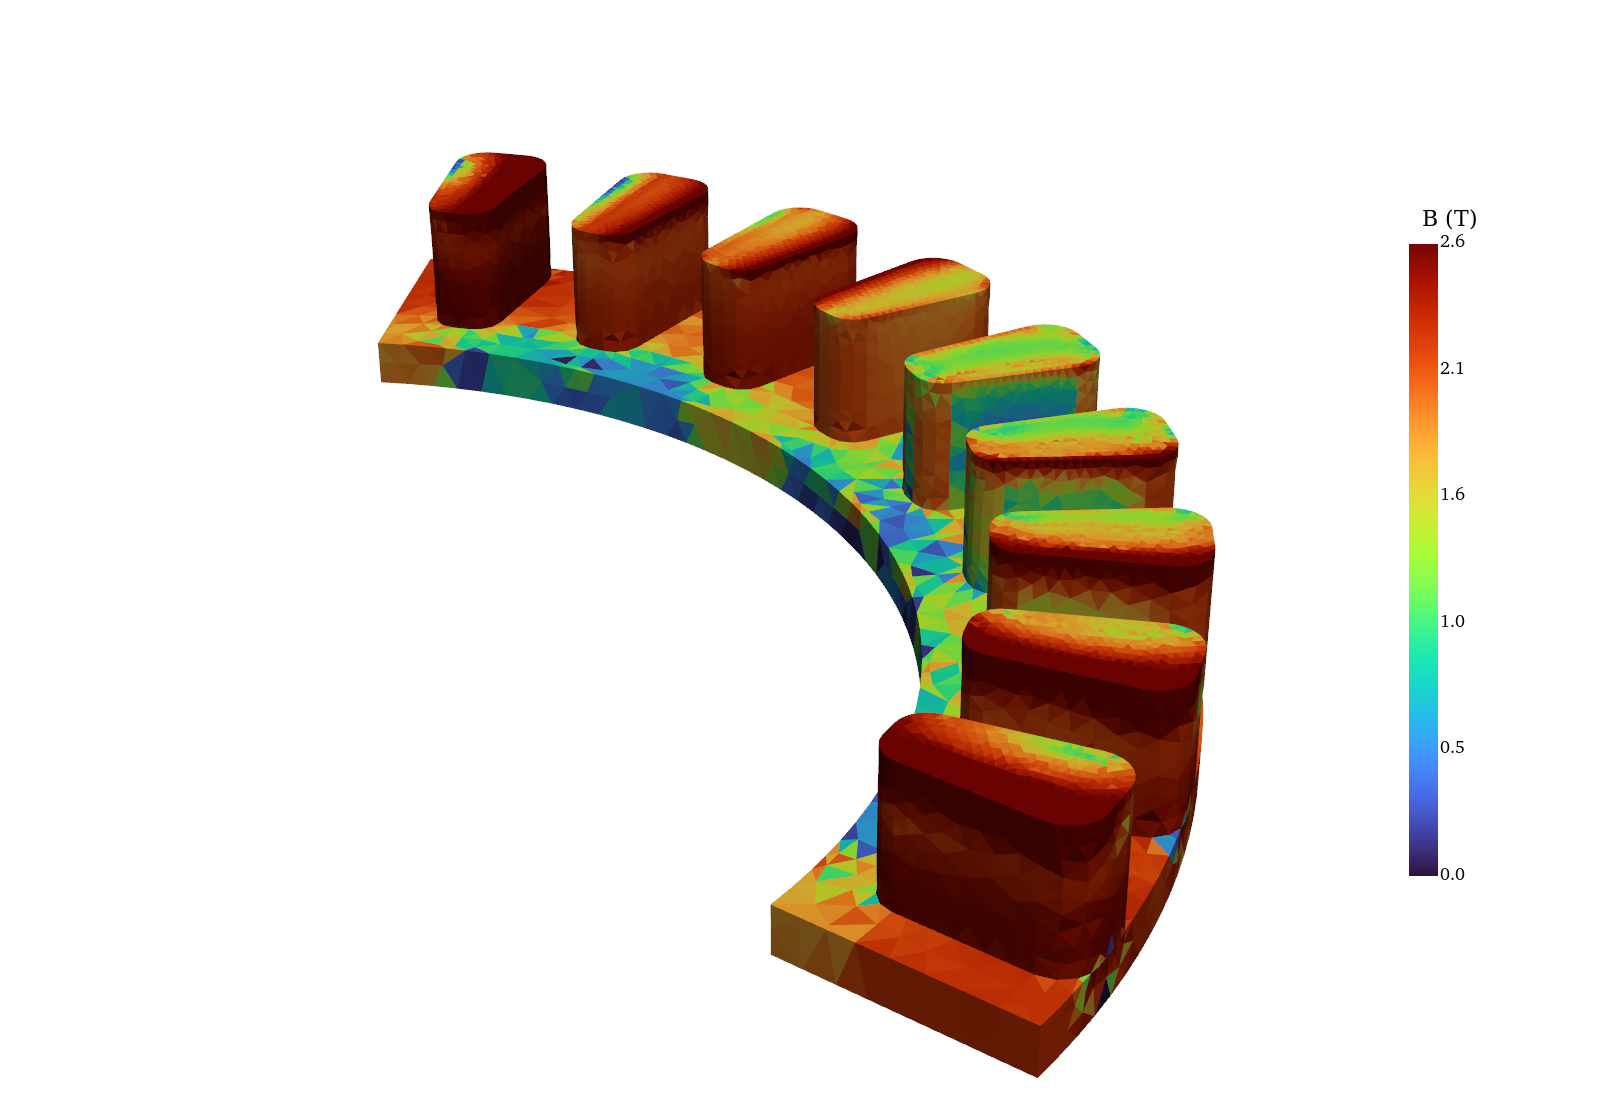
\includegraphics[width=0.49\columnwidth,trim=330 60 0 120,clip]{r3d_statorB_i250.png}}
\caption{$|B|$ on the surfaces of the stator core over one periodic sector (coils hidden). Colour scale \SIrange{0}{2.6}{T}.}
\label{fig:statorB}
\end{figure}

\begin{figure}[!t]
\centering
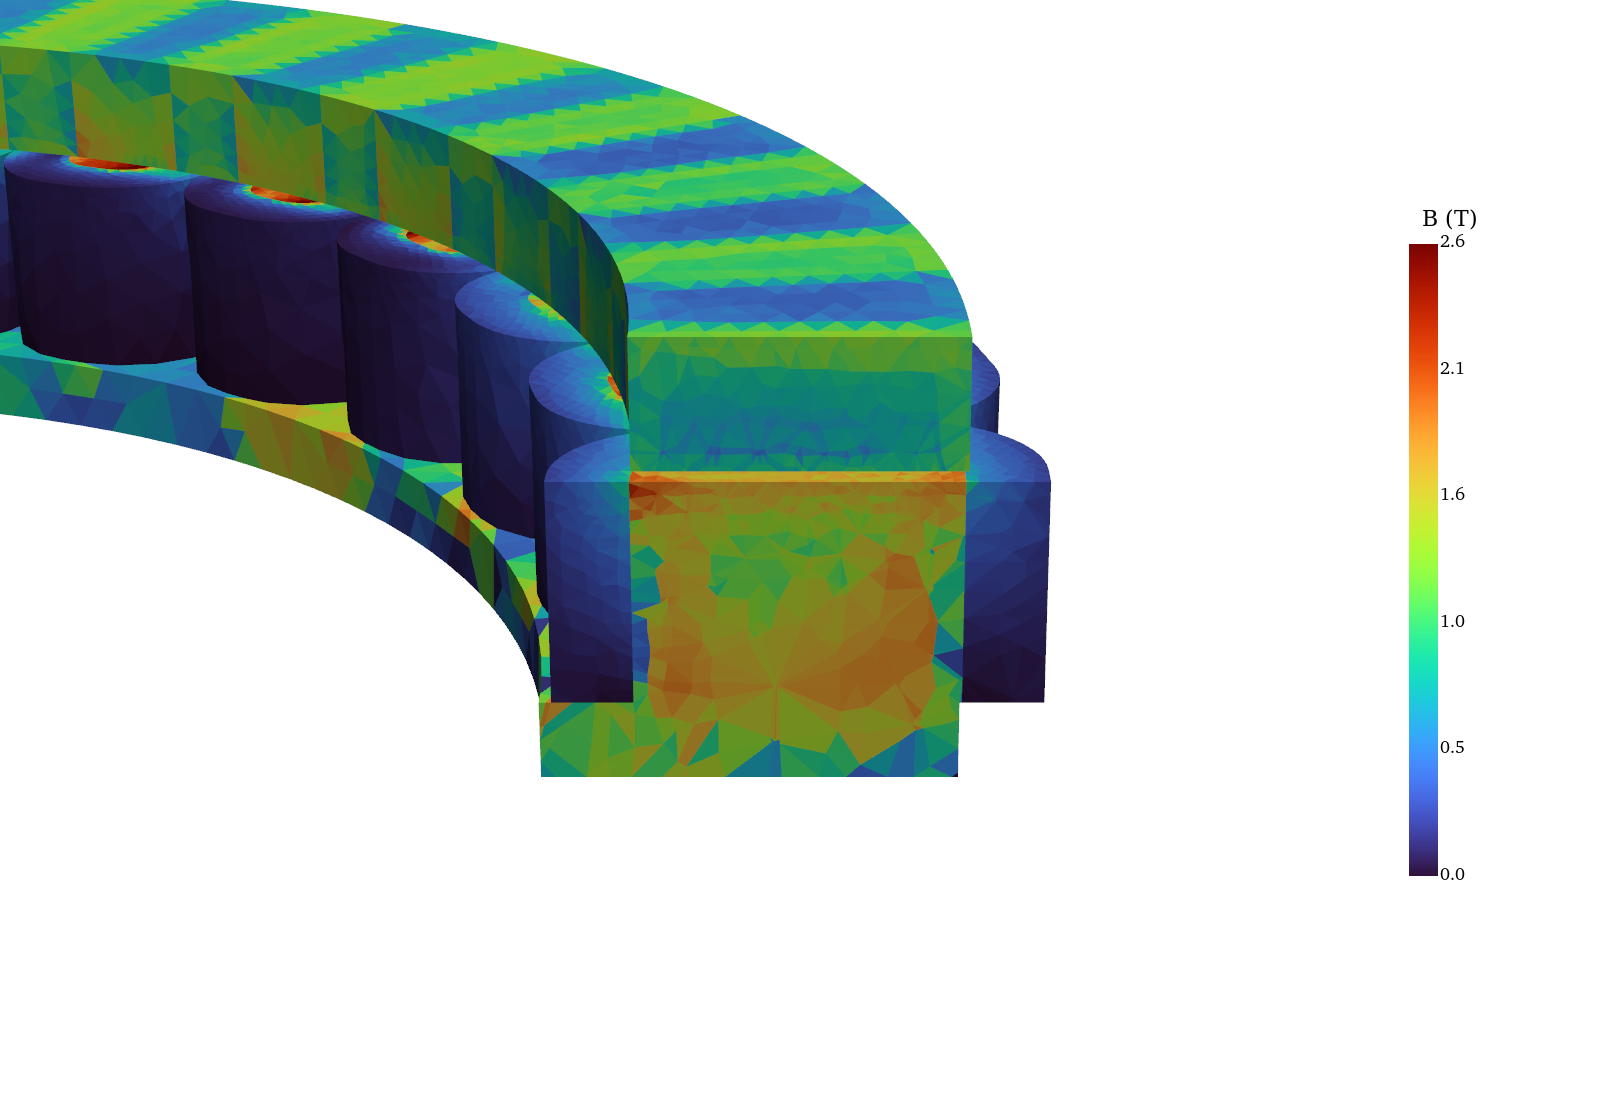
\includegraphics[width=\columnwidth,trim=0 260 0 0,clip]{r3d_clip.png}
\caption{Model cut through the centre plane of a tooth at \SI{250}{A}, showing $|B|$ inside the core, coils and magnets.}
\label{fig:clip}
\end{figure}

\begin{figure}[!t]
\centering
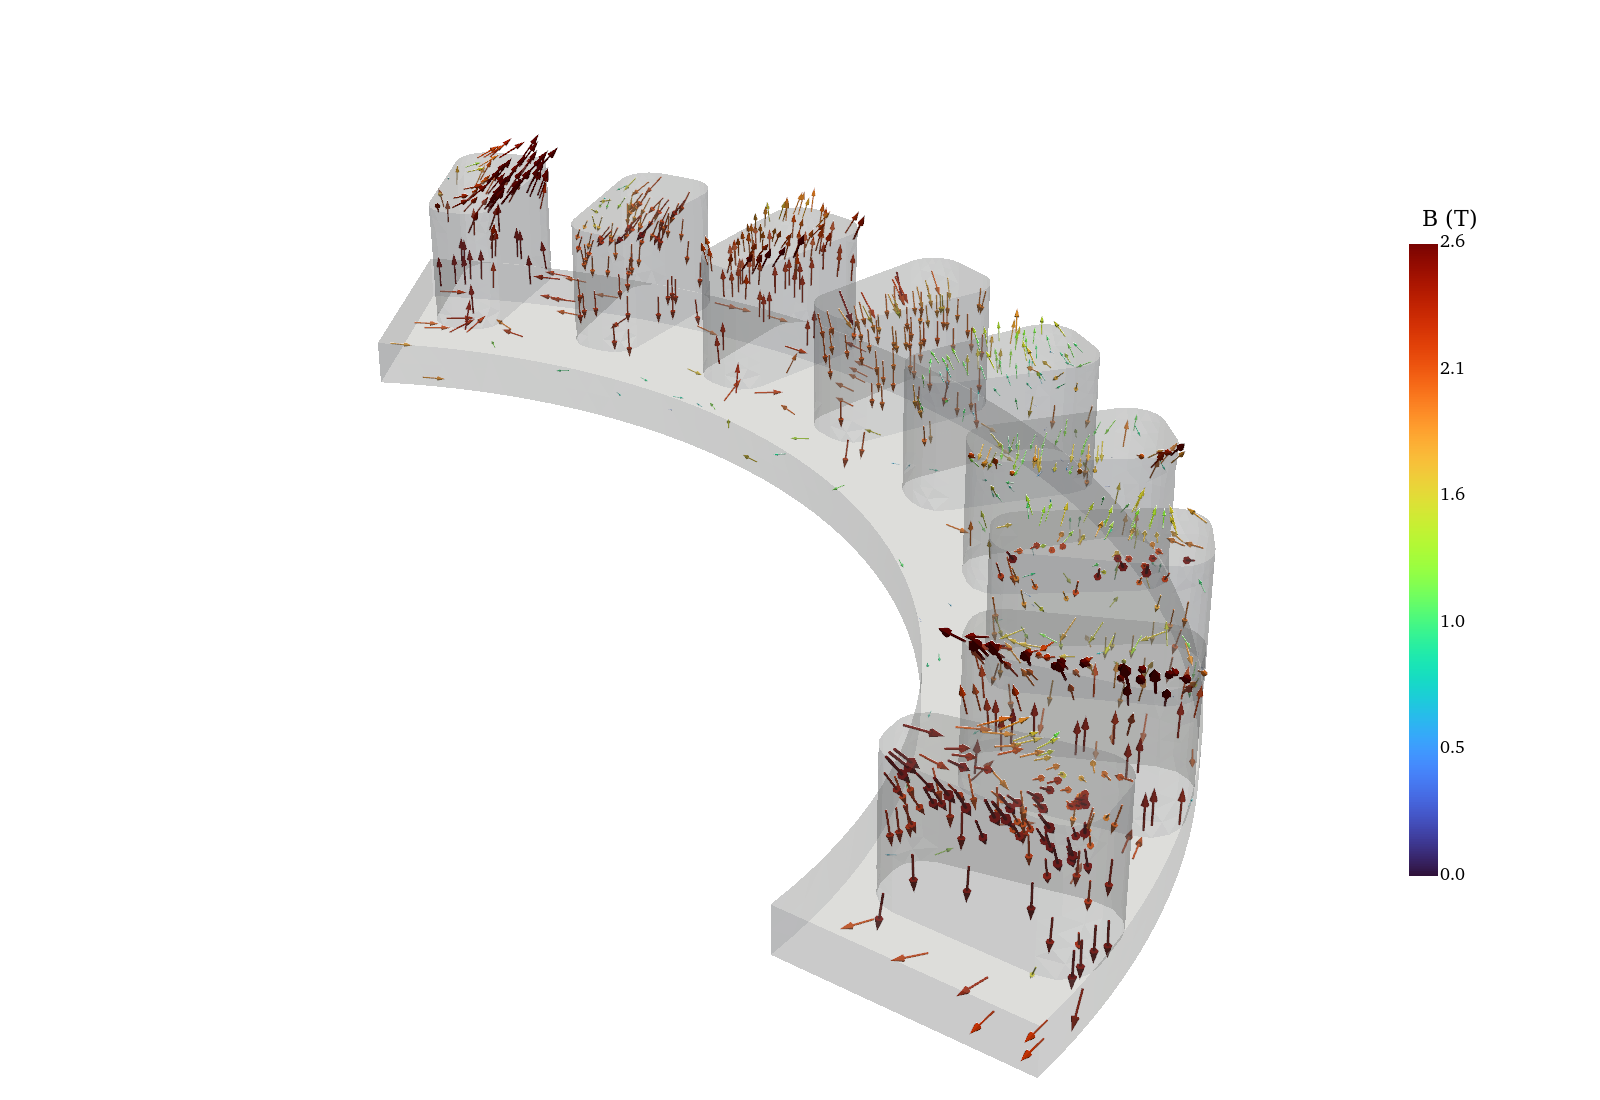
\includegraphics[width=\columnwidth,trim=330 60 0 100,clip]{r3d_vectors.png}
\caption{Flux-density vectors in the stator core at \SI{250}{A} (every 25th element shown, scaled and coloured by $|B|$).}
\label{fig:vectors}
\end{figure}

\subsection{Two-dimensional slices of the 3-D solution}
For direct comparison with the multi-slice literature \cite{parviainen2005,gieras2008}, \cref{fig:tz250,fig:tz0} show the 3-D solution sampled on cylindrical surfaces at three radii and unrolled into the $(r\theta,z)$ plane. Unlike \cref{fig:quasi3d}, these slices include the radial flux leaving each surface. At the inner radius the slot pitch is smallest and the teeth saturate first. At \SI{250}{A} the flux lines show armature reaction displacing flux toward one side of each pole. The Halbach rotor closes the flux path inside the magnet layer: the tangential pieces carry flux circumferentially, and the field behind the magnets, in the non-magnetic carrier, is weak.

\begin{figure*}[!t]
\centering
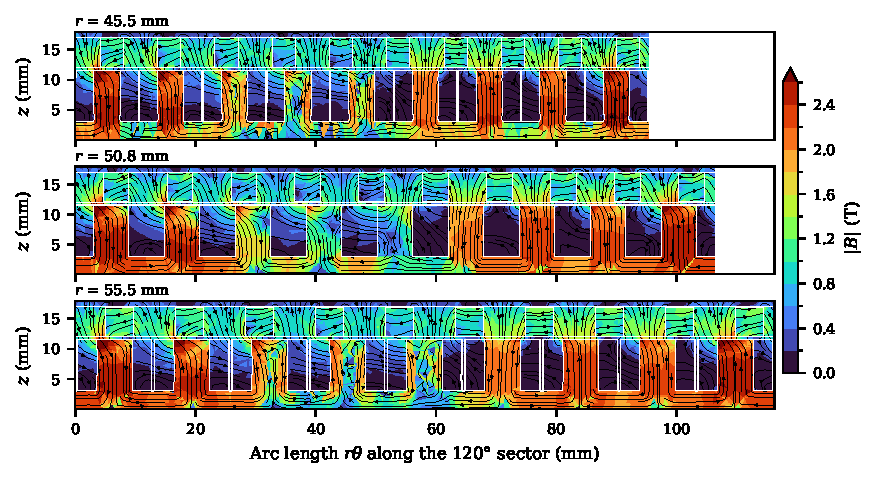
\includegraphics[width=\textwidth]{slices_tz_i250.pdf}
\caption{3-D solution at \SI{250}{A} ($q$ axis): $|B|$ and in-plane flux lines on cylindrical surfaces at $r=45.5$, 50.75 and \SI{55.5}{mm}, unrolled over the 120\si{\degree} sector. White lines outline core, coils and magnets.}
\label{fig:tz250}
\end{figure*}

\begin{figure*}[!t]
\centering
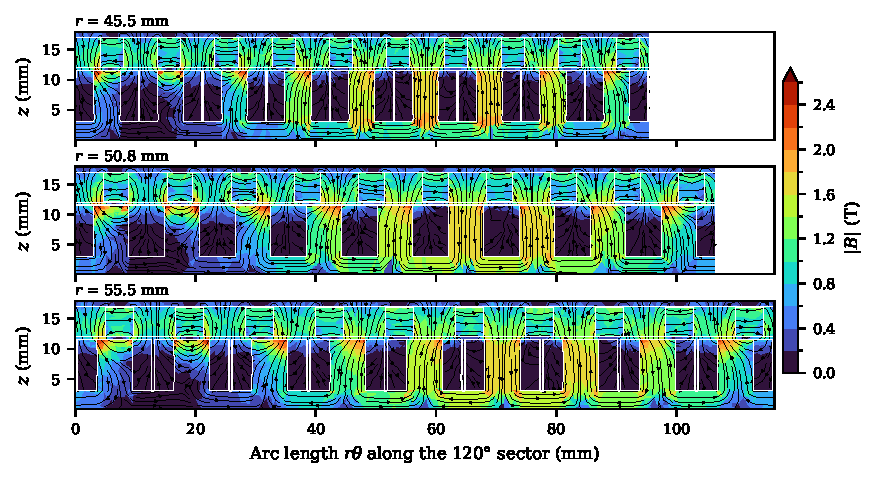
\includegraphics[width=\textwidth]{slices_tz_i0.pdf}
\caption{As \cref{fig:tz250}, at no load.}
\label{fig:tz0}
\end{figure*}

\Cref{fig:rz} shows radial--axial sections through a tooth centre and a slot centre. These views are impossible in a 2-D slice model. They show fringing flux leaving the magnet ends at $R_i$ and $R_o$, the flux in the tooth overhang beyond the magnet annulus, and the end-region leakage that the 2-D model misses.

\begin{figure*}[!t]
\centering
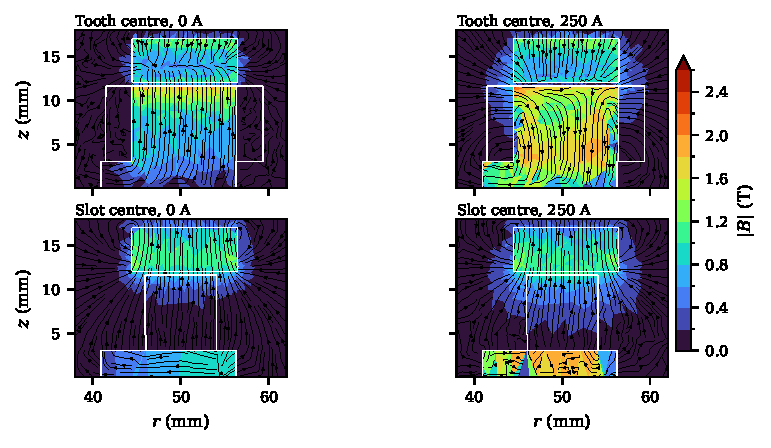
\includegraphics[width=0.9\textwidth]{sections_rz.pdf}
\caption{Radial--axial sections of the 3-D solution through a tooth centre (top) and a slot centre (bottom), at no load (left) and \SI{250}{A} (right).}
\label{fig:rz}
\end{figure*}

\Cref{fig:polar} shows the true geometry in planes normal to the axis: \SI{1}{mm} below the tooth tips, and through the middle of the magnets. The Halbach pattern is visible in the magnet plane: the tangential pieces carry flux circumferentially between the axial pieces.

\begin{figure*}[!t]
\centering
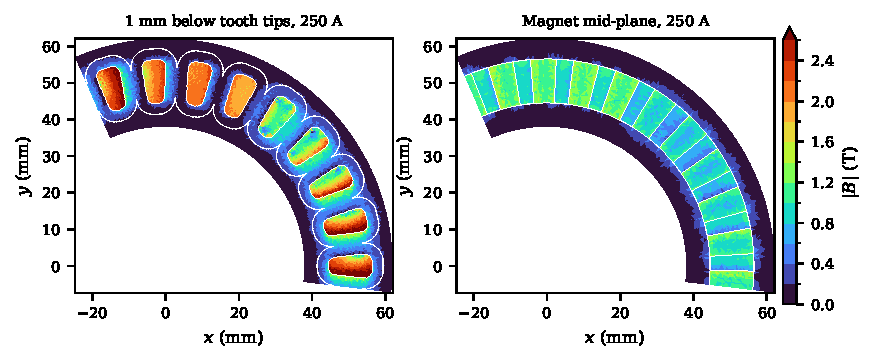
\includegraphics[width=0.85\textwidth]{polar_planes.pdf}
\caption{$|B|$ in planes normal to the axis at \SI{250}{A}: (left) \SI{1}{mm} below the tooth tips, (right) magnet mid-plane.}
\label{fig:polar}
\end{figure*}

\subsection{Air-gap field}
\Cref{fig:gapmap} maps $B_z$ on the gap mid-plane over the sector, and \cref{fig:gapprof} extracts the profile at the mean radius, its harmonic content, and the radial profile at a pole centre. The Halbach rotor gives a nearly trapezoidal-sinusoidal no-load field with a strong fundamental. Slot openings superimpose the expected modulation. The radial profile drops over roughly 1--\SI{2}{mm} at each end of the annulus, which corresponds to the \SI{2}{\percent} no-load fringing loss relative to 2-D.

\begin{figure*}[!t]
\centering
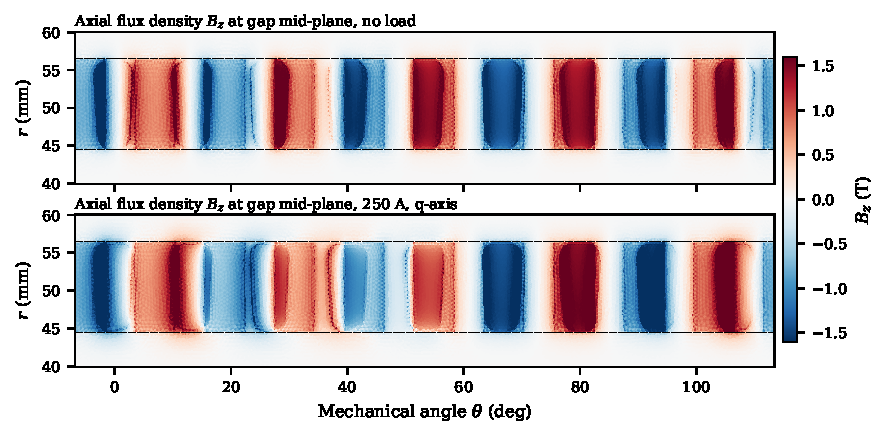
\includegraphics[width=\textwidth]{gap_map.pdf}
\caption{Axial flux density $B_z$ on the air-gap mid-plane, unrolled in $(\theta,r)$, at no load (top) and \SI{250}{A} (bottom). Dashed lines: magnet radii $R_i$ and $R_o$.}
\label{fig:gapmap}
\end{figure*}

\begin{figure*}[!t]
\centering
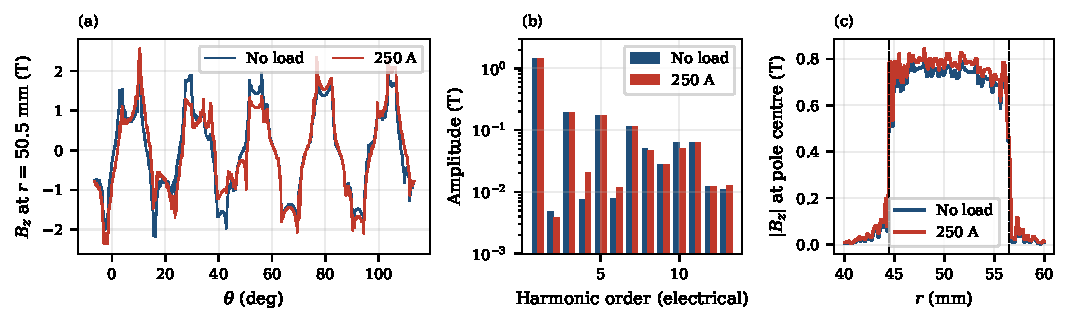
\includegraphics[width=\textwidth]{gap_profiles.pdf}
\caption{Air-gap field. (a) $B_z$ against angle at $r=\SI{50.5}{mm}$; (b) harmonic spectrum (electrical orders); (c) $|B_z|$ against radius at the centre of an axially magnetised piece.}
\label{fig:gapprof}
\end{figure*}

\subsection{Torque, flux linkage and axial force}
\Cref{fig:sweep} and \cref{tab:sweep} give torque, axial pull and stator flux linkage from 0 to \SI{300}{A} on the $q$ axis, together with the effect of current advance at \SI{250}{A}. The no-load flux linkage is $\psi_m=\SI{8.62}{mWb}$, so the linear torque constant is $\frac32 p\psi_m=\SI{0.194}{\newton\metre\per\ampere}$. At \SI{250}{A} the 3-D torque is 86\,\% of the linear value, and at \SI{300}{A} it is 80\,\%: saturation, not magnet strength, sets the peak torque. Unlike a steel-backed rotor, the axial pull falls with $q$-axis current, because armature reaction weakens the main flux under half of each pole. Current advance reduces torque monotonically, so the maximum-torque-per-ampere angle is close to the $q$ axis.
\begin{figure*}[!t]\centering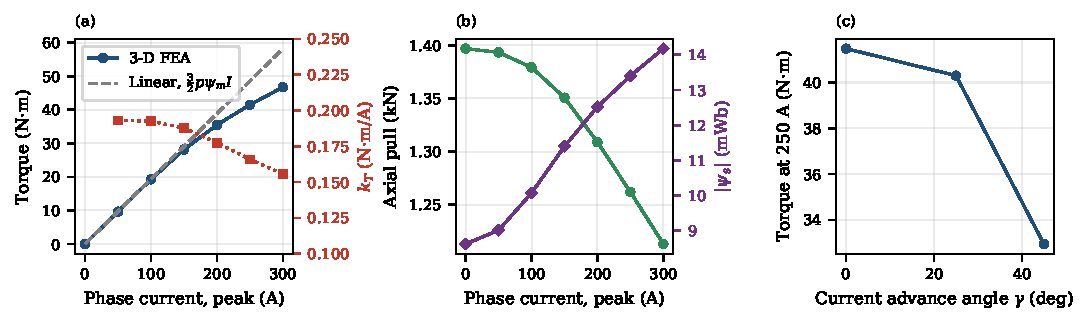
\includegraphics[width=\textwidth]{sweep.pdf}
\caption{TREN-V4 v4b performance from the 3-D model. (a) Torque and torque constant against $q$-axis current, with the linear (unsaturated) extrapolation; (b) axial magnetic pull and stator flux-linkage magnitude; (c) torque against current advance angle at \SI{250}{A}.}\label{fig:sweep}\end{figure*}
\begin{table}[!t]\caption{3-D results against $q$-axis current (v4b, ideal materials)}\label{tab:sweep}\centering\footnotesize
\begin{tabular}{@{}rrrrr@{}}\toprule $I$ (A) & $T$ (\Nm) & $k_T$ (\Nm/A) & $F_z$ (kN) & $|\psi_s|$ (mWb)\\\midrule
0 & 0.03 & -- & 1.40 & 8.62\\
50 & 9.66 & 0.193 & 1.39 & 9.01\\
100 & 19.26 & 0.193 & 1.38 & 10.07\\
150 & 28.16 & 0.188 & 1.35 & 11.40\\
200 & 35.48 & 0.177 & 1.31 & 12.52\\
250 & 41.48 & 0.166 & 1.26 & 13.40\\
300 & 46.72 & 0.156 & 1.21 & 14.18\\
\bottomrule\end{tabular}\end{table}



\subsection{Torque--speed envelope and efficiency}
\Cref{fig:tn} shows the motor torque--speed envelope at a \SI{48}{V} bus with an efficiency map underneath. The envelope comes from a $dq$ model whose $q$-axis torque follows the 3-D sweep of \cref{tab:sweep}, i.e.\ $\psi_\mathrm{eff}(I)=T(I)/(\tfrac32pI)$. It uses $\psi_m=\SI{8.62}{mWb}$, $L_d=L_q=\SI{52}{\micro H}$, $R=\SI{37.5}{m\ohm}$ (\SI{100}{\celsius}), modulation index 0.96, $|i_d|\le\SI{120}{A}$, and the minimum-current $(i_d,i_q)$ pair at every operating point. The losses are copper loss with a Dowell AC factor $1+0.3(f/\SI{550}{Hz})^2$, core loss scaled from the motor-thread Steinmetz estimate, \SI{10}{W} of rotor eddy loss at \SI{2200}{rpm} scaling with $n^2$, and an assumed \SI{0.02}{\Nm} bearing drag. The map is motor-only: inverter and gearbox losses are excluded.
The constant-torque region extends to about \SI{90}{rad/s} (\SI{14}{rad/s} at the output), after which field weakening holds useful torque to the edge of the plot. Peak efficiency is 94\,\% at moderate torque and \SIrange{150}{220}{rad/s}. In the high-torque, low-speed region used in stance, efficiency is low (below 50\,\%) because copper loss dominates. This is the reason the thermal limit, not the envelope, governs locomotion.

\begin{figure}[!t]
\centering
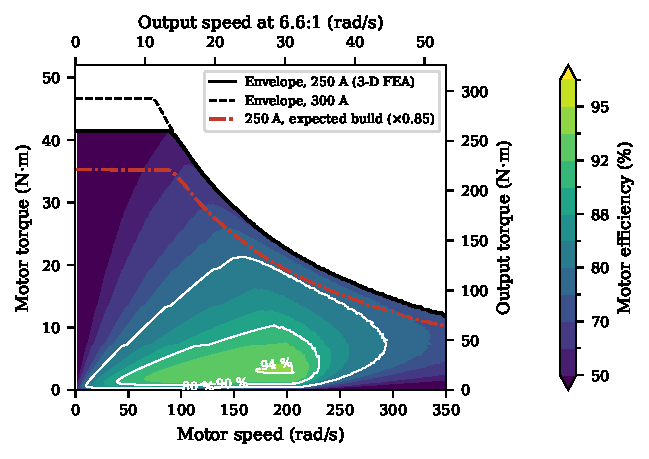
\includegraphics[width=\columnwidth]{tn_eff.pdf}
\caption{Motor torque--speed envelope at \SI{48}{V} (\SI{250}{A}, solid; \SI{300}{A}, dashed; expected built motor at 0.85$\times$, dash-dot) over the motor efficiency map, with output-shaft axes for the 6.6:1 reduction ($\eta=0.95$).}
\label{fig:tn}
\end{figure}

\subsection{Thermal endurance: constant versus sinusoidal current}
The winding-temperature limit is evaluated with the four-node lumped model of the motor design thread: winding, core, housing and ambient. The stator is v0.4.10 ($R_{20}=\SI{28.5}{m\ohm}$, winding capacity about \SI{88}{J/K}), the housing-to-air resistance is \SI{1}{K/W}, and each run starts at \SI{40}{\celsius}. Two duty types are compared in \cref{fig:thermal,tab:thermal}:
\begin{itemize}
\item \emph{constant peak}: the current amplitude is held at $I$, as in a static hold or a sustained push, so copper loss is $\tfrac32I^2R$;
\item \emph{sinusoidal}: the torque command swings sinusoidally between $+I$ and $-I$ with a \SI{0.4}{s} stride period, as in a locomotion gait. Mean copper loss is then half as large.
\end{itemize}
The sinusoidal case is the more relevant one for running. It reaches \SI{150}{\celsius} after about \SI{8}{s} at \SI{250}{A} and \SI{16}{s} at \SI{200}{A}, compared with \SI{3.4}{s} and \SI{5.9}{s} at constant current. The ratio grows from about 2.4 at high current to 3 or more at low current, because the winding and core thermal capacitances absorb the oscillating part of the loss.

\begin{figure}[!t]
\centering
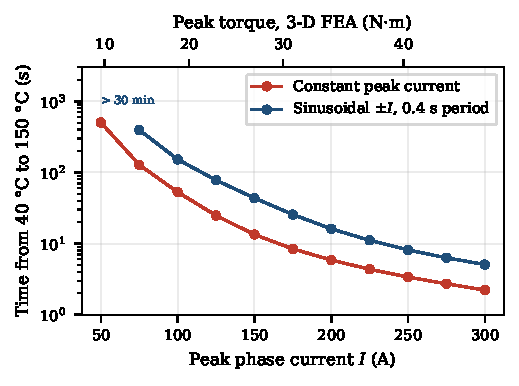
\includegraphics[width=\columnwidth]{thermal_t150.pdf}
\caption{Time for the winding to rise from \SI{40}{\celsius} to \SI{150}{\celsius} against peak current, for constant current and for a sinusoidal $\pm I$ trajectory with \SI{0.4}{s} period. Top axis: corresponding peak torque from the 3-D model.}
\label{fig:thermal}
\end{figure}

\begin{table}[!t]
\caption{Time from \SI{40}{\celsius} to \SI{150}{\celsius} winding temperature (s)}\label{tab:thermal}
\centering\footnotesize
\begin{tabular}{@{}rrrr@{}}
\toprule
$I$ (A, peak) & Constant & Sinusoidal $\pm I$ & Ratio\\
\midrule
50 & 502 & $>$1800 & --\\
75 & 128 & 395 & 3.1\\
100 & 52.9 & 152 & 2.9\\
125 & 24.8 & 77.7 & 3.1\\
150 & 13.4 & 43.5 & 3.3\\
175 & 8.4 & 25.6 & 3.0\\
200 & 5.9 & 16.1 & 2.8\\
225 & 4.4 & 11.1 & 2.5\\
250 & 3.4 & 8.1 & 2.4\\
275 & 2.7 & 6.3 & 2.3\\
300 & 2.2 & 5.1 & 2.3\\
\bottomrule
\end{tabular}
\end{table}


\subsection{Magnet working point}
\Cref{fig:demag} shows the opposing field on the magnet surfaces at \SI{250}{A}, and \cref{fig:stats}(b) its volume distribution. The highest values sit on the stator-facing corners of the tangential pieces. In the core of the tangential pieces the 99.9th percentile is \SI{1.25}{MA/m}, against \SI{1.03}{MA/m} for the axial pieces. With the criterion $H_{op}\le0.9H_{cJ}(T)$, N52SH is safe only to about \SI{36}{\celsius} in the tangential pieces. N50UH (about \SI{72}{\celsius}) or N48EH (about \SI{98}{\celsius}) is required, which lowers $B_r$ and, through \cref{fig:sens}, torque.

\begin{figure}[!t]
\centering
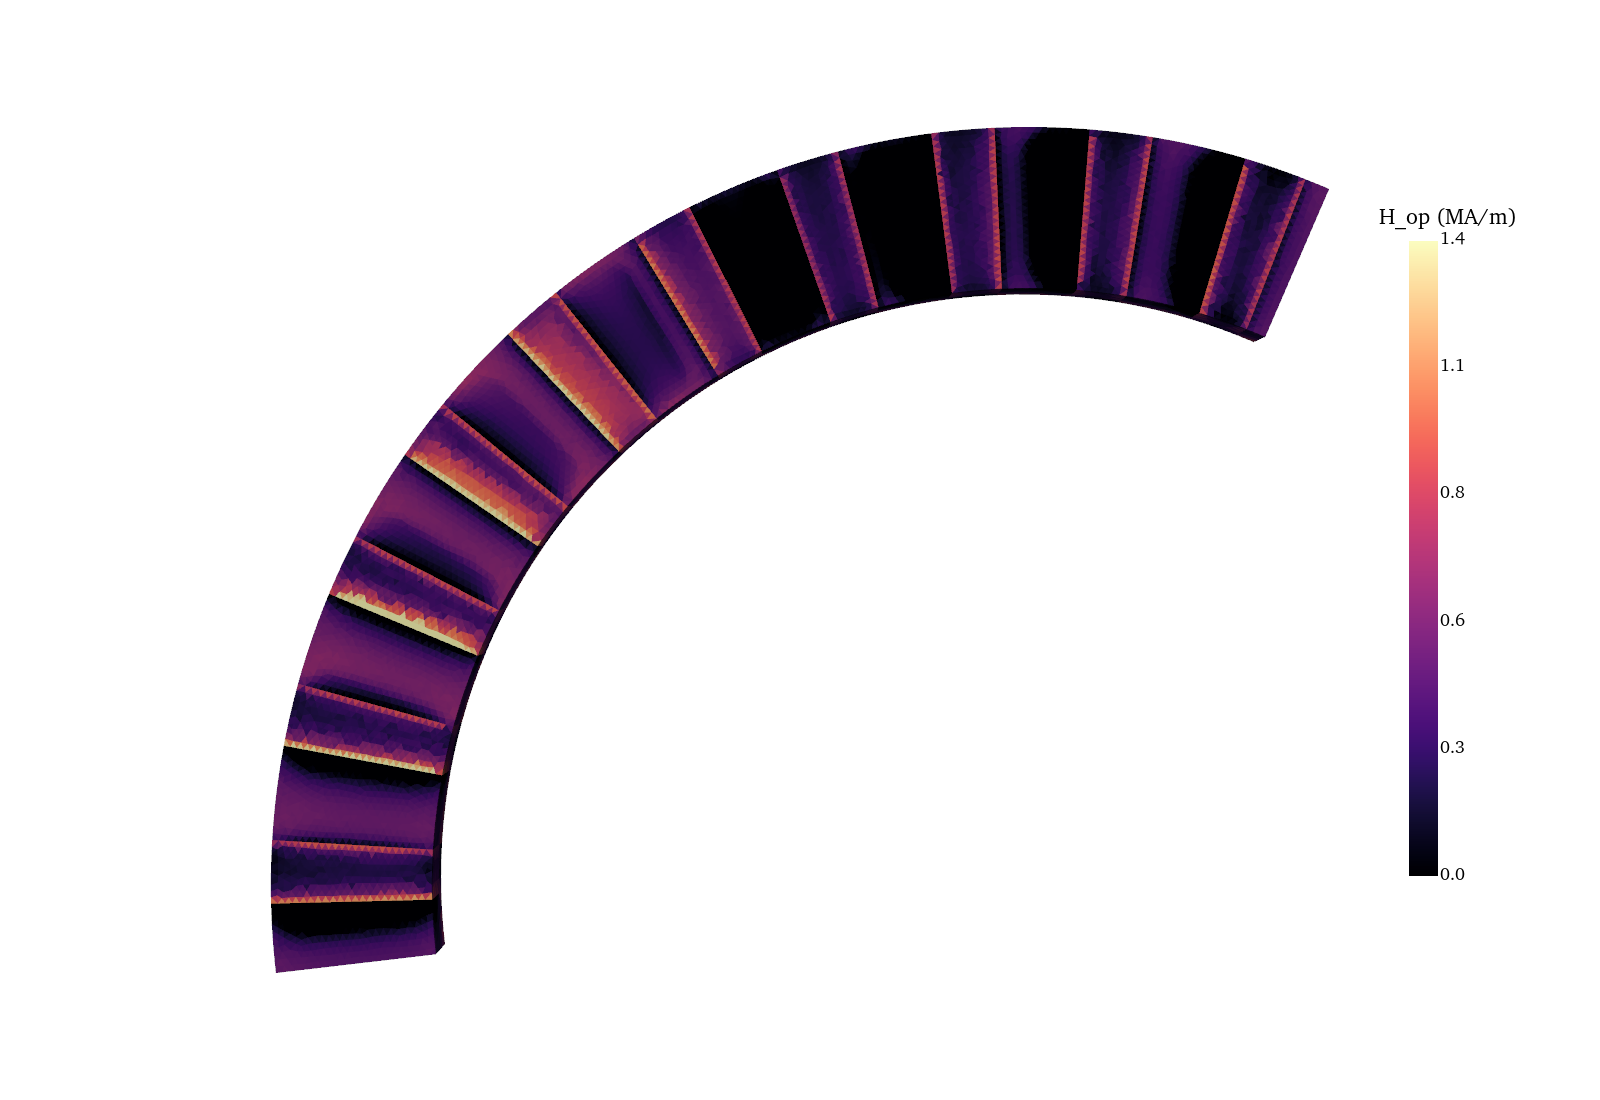
\includegraphics[width=\columnwidth,trim=200 60 0 100,clip]{r3d_magnet_Hop.png}
\caption{Opposing field $H_{op}$ on the magnet surfaces at \SI{250}{A}, viewed from the stator side (mirror image of the top view).}
\label{fig:demag}
\end{figure}

\begin{figure*}[!t]
\centering
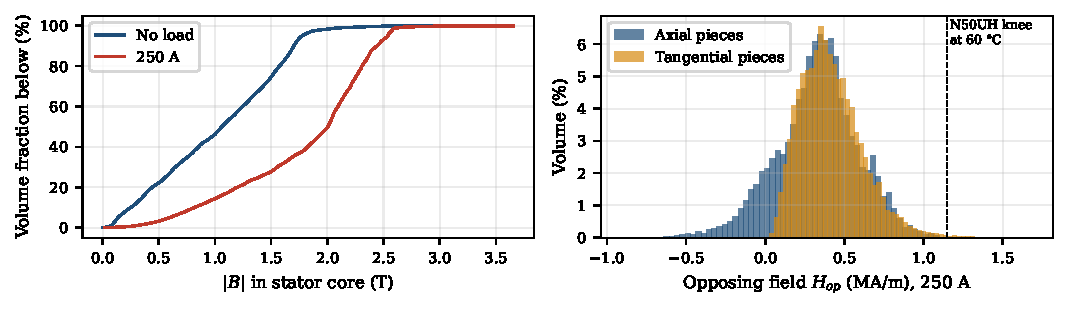
\includegraphics[width=0.9\textwidth]{stats.pdf}
\caption{(a) Volume-weighted cumulative distribution of $|B|$ in the stator core; (b) volume distribution of the opposing field in axial and tangential magnet pieces at \SI{250}{A}, with the N50UH knee ($0.9H_{cJ}$) at \SI{60}{\celsius}.}
\label{fig:stats}
\end{figure*}

\subsection{Design evolution}
\Cref{fig:evol} places v4b in the sequence of designs analysed with the same tool. Closing the gap from 0.7 to \SI{0.4}{mm} added \SI{9}{\percent}. The Halbach array added a further \SI{15}{\percent} over the tube-rotor baseline while reducing rotor mass. A \SI{1}{mm} 40Cr back ring behind the Halbach array adds another \SI{5}{\percent}.

\begin{figure}[!t]
\centering
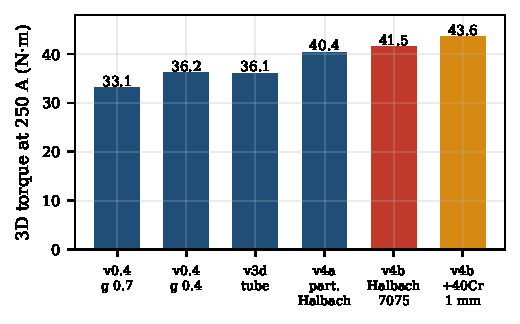
\includegraphics[width=\columnwidth]{evolution.pdf}
\caption{3-D torque at \SI{250}{A} for successive TREN-V4 design variants (ideal materials, \SI{20}{\celsius}).}
\label{fig:evol}
\end{figure}

\FloatBarrier
\section{Expected Torque of the Built Motor}\label{sec:realistic}
The \SI{41.5}{\Nm} result assumes ideal materials and geometry. \Cref{fig:sens} shows 3-D sensitivity runs on the same mesh. The largest single effect is the core stacking factor. The model applies the solid Hiperco~50 curve to the whole core volume, but a \SI{0.1}{mm} tape-wound core is typically around \SI{90}{\percent} metal. A stacking factor of 0.92 costs \SI{4.0}{\percent}, applied as $B_\mathrm{eff}=k_sB(H)+(1-k_s)\mu_0H$. A combined realistic build (stacking 0.92, \SI{0.05}{mm} joints between Halbach pieces, \SI{0.45}{mm} gap, $H$ increased by 1.5 for cutting damage) gives \SI{38.6}{\Nm} ($-\SI{6.9}{\percent}$).

\begin{figure}[!t]
\centering
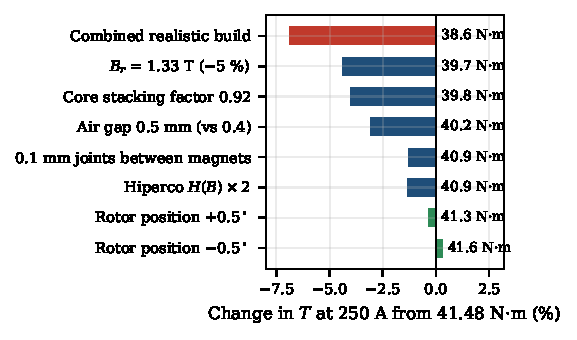
\includegraphics[width=\columnwidth]{sensitivity.pdf}
\caption{3-D sensitivity of the \SI{250}{A} torque to manufacturing and material deviations, from \SI{41.48}{\Nm}.}
\label{fig:sens}
\end{figure}

\Cref{tab:budget} combines the three independent factors. Build effects come from the sensitivity runs. The load-side gap between FEA and measured shaft torque comes from the benchmark of \cref{sec:verify}, which anchored no-load flux to measurement and so does not double-count build effects. Magnet temperature uses the measured $B_r$ sensitivity, $\partial T/\partial B_r\approx0.88\,T/B_r$, with $-\SI{0.11}{\percent/\celsius}$ for NdFeB.

\begin{table}[!t]
\caption{Expected torque at \SI{250}{A}, v4b rotor}\label{tab:budget}
\centering\footnotesize
\begin{tabular}{@{}lccc@{}}
\toprule
Factor & Low & Central & High\\
\midrule
Ideal 3-D FEA (\Nm) & \multicolumn{3}{c}{41.5}\\
Build: stacking, joints, gap, core & 0.91 & 0.93 & 0.95\\
FEA-to-measured load gap & 0.92 & 0.94 & 0.97\\
Magnet temperature (80/50/\SI{20}{\celsius}) & 0.94 & 0.97 & 1.00\\
\midrule
\textbf{Expected torque (\Nm)} & \textbf{32.7} & \textbf{35.2} & \textbf{38.2}\\
Output at 6.6:1, $\eta=0.95$ (\Nm) & 205 & 221 & 240\\
\bottomrule
\end{tabular}
\end{table}

The central estimate, \SI{35}{\Nm}, is \SI{15}{\percent} below the ideal result but still meets the \SI{180}{\Nm} output target with margin. The three most useful measurements, in order, are: the core vendor's stacking factor and a $B$--$H$ curve measured on an annealed tape core (about $\pm\SI{4}{\percent}$); the magnet lot's $B_r$ and grade (about $\pm\SI{4}{\percent}$); and a locked-rotor torque test of the first stator from 50 to \SI{250}{A}. The test calibrates the whole chain in one step, after which the FEA can be used with a single correction factor.

\FloatBarrier
\section{Magnet Grade Selection and Rotor Temperature}\label{sec:grades}
\begin{figure*}[!t]
\centering
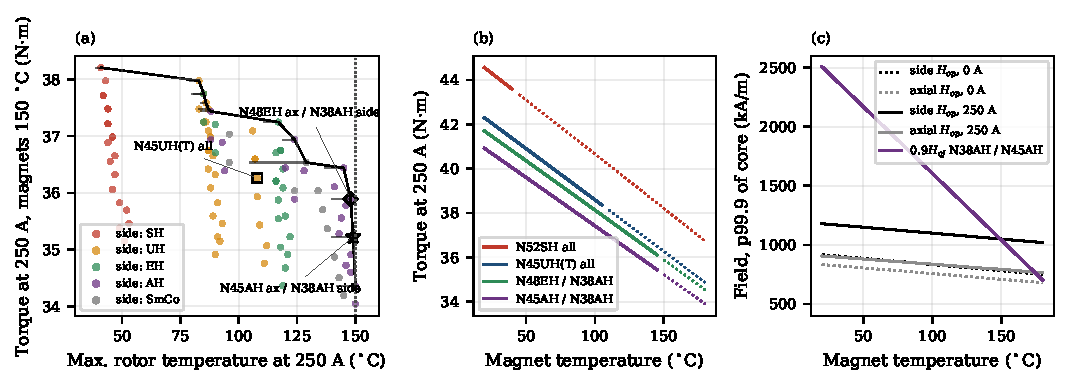
\includegraphics[width=\textwidth]{grades.pdf}
\caption{Magnet grade selection, 40Cr-backed v4b rotor, ideal materials. (a) All 100 axial/side grade pairs: torque at \SI{250}{A} with \SI{150}{\celsius} magnets against the highest magnet temperature that passes the knee criterion at \SI{250}{A}. The black line is the Pareto front; the whiskers reach the 95\,\% (5th-percentile) temperature from Monte Carlo. (b) Torque against magnet temperature at \SI{250}{A}; dotted where the pair would be partially demagnetised. (c) Recommended pair: 99.9th-percentile reverse field in the side and axial pieces against the knee of N38AH/N45AH.}
\label{fig:grades}
\end{figure*}

The rotor is now fixed as the v4b Halbach array on a \SI{1}{mm} quenched-and-tempered 40Cr back ring. 4140 or 4340 steel can be used for the ring instead. All three are medium-carbon Cr(--Mo/Ni) alloy steels with similar saturation. The ring is modelled with an estimated Q\&T 40Cr $B$--$H$ curve, and 2-D runs showed the ring material changes torque by less than \SI{1}{\percent}. The stator winding is limited to \SI{150}{\celsius}. A magnet set that tolerates \SI{150}{\celsius} at full current therefore removes the rotor as a separate thermal limit. This section asks which magnet grade, or pair of grades, gives the most torque under that constraint.

\subsection{N45UH(T) on the 40Cr ring}
Direct 3-D solves with N45UH-class magnets ($B_r=\SI{1.35}{T}$ at \SI{20}{\celsius}, $-\SI{0.12}{\percent/K}$, from the Arnold GB45UH datasheet) give \SI{42.2}{\Nm} at \SI{250}{A} with \SI{20}{\celsius} magnets, and \SI{39.6}{\Nm} at \SI{80}{\celsius}. The catalogue rating of \SI{180}{\celsius} for this class applies to a magnet in its own field at a moderate permeance coefficient. In the Halbach array the side (tangentially magnetised) pieces also carry the reverse field of their neighbours and of the stator. The 99.9th percentile of that field in their core is \SI{0.97}{MA/m} at no load and \SI{1.23}{MA/m} at \SI{250}{A}. With the knee criterion $H_{op}\le0.9H_{cJ}(T)$, N45UH(T) is limited to about \SI{108}{\celsius} at \SI{250}{A}.

\begin{figure*}[!t]
\centering
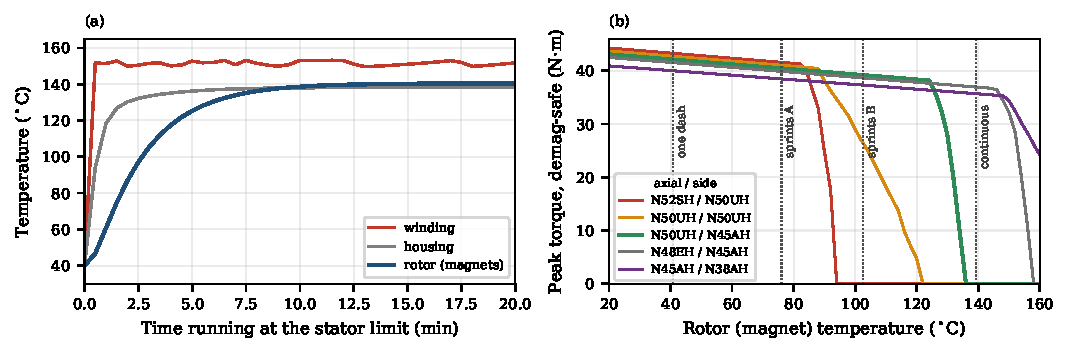
\includegraphics[width=\textwidth]{rotor_thermal.pdf}
\caption{(a) Winding, housing and rotor temperature when the motor runs continuously at its \SI{150}{\celsius} winding limit, starting from \SI{40}{\celsius}. (b) Peak torque available without demagnetisation against rotor temperature for candidate pairs (axial/side), with current limited where needed to stay below the knee (ideal materials). Dotted lines mark the rotor temperatures of \cref{tab:rotorT}: one dash; repeated sprints resting to \SI{70}{\celsius} (A) and to \SI{100}{\celsius} (B); continuous running at the limit.}
\label{fig:rotorT}
\end{figure*}

\subsection{Surrogate model and Monte Carlo search}
The magnets are linear ($\mu_r=1.05$), so the field at any point in them depends on three inputs: the remanence of the axial pieces $B_{r,a}$, the remanence of the side pieces $B_{r,t}$ and the current. Nine 3-D solves were run on one mesh, spanning $B_{r,a},B_{r,t}\in[1.0,1.3]$\,T and $I\in\{0,150,250\}$\,A. At each of \num{2e5} fixed sample points in the magnets, $\bm{M}\cdot\bm{B}$ was fitted to $\{1,B_{r,a},B_{r,t},I,I^2\}$. Torque at \SI{250}{A} was fitted bilinearly in the two remanences. The surrogate was checked against FEA it was not fitted to:
\begin{itemize}
\item a held-out solve at $(1.18,1.12)$\,T, \SI{250}{A}: the field percentiles are within \SI{0.6}{\percent} and torque within \SI{0.2}{\percent};
\item the six independent N45UH(T) solves at \SIlist{1.35;1.25}{T}, outside the fitted range: the field percentiles are within \SI{0.7}{\percent} and torque within \SI{0.3}{\percent}.
\end{itemize}
Each evaluation then costs milliseconds instead of 20 minutes, which makes an exhaustive search with Monte Carlo tolerance analysis possible.

\begin{table}[!t]
\caption{Magnet grade catalogue (typical $B_r$, minimum $H_{cJ}$ at \SI{20}{\celsius})}\label{tab:catalogue}
\centering\scriptsize\setlength{\tabcolsep}{4pt}
\begin{tabular}{@{}lccccc@{}}
\toprule
Grade & $B_r$ & $H_{cJ}$ & $\alpha_{B_r}$ & $\beta_{H_{cJ}}$ & $H_k/H_{cJ}$\\
 & (T) & (kA/m) & (\si{\percent/K}) & (\si{\percent/K}) & \\
\midrule
N52SH & 1.43 & 1592 & $-0.12$ & $-0.55$ & 0.90\\
N50SH & 1.40 & 1592 & $-0.12$ & $-0.55$ & 0.90\\
N50UH $^\dagger$ & 1.40 & 1990 & $-0.12$ & $-0.50$ & 0.90\\
N48UH & 1.37 & 1990 & $-0.12$ & $-0.52$ & 0.90\\
N45UH(T) $^\dagger$ & 1.35 & 2149 & $-0.12$ & $-0.47$ & 0.90\\
N48EH $^\dagger$ & 1.37 & 2388 & $-0.12$ & $-0.48$ & 0.90\\
N42EH & 1.30 & 2388 & $-0.12$ & $-0.50$ & 0.90\\
N45AH $^\dagger$ & 1.33 & 2786 & $-0.12$ & $-0.45$ & 0.90\\
N38AH & 1.24 & 2786 & $-0.11$ & $-0.45$ & 0.90\\
Sm$_2$Co$_{17}$ 32H & 1.13 & 1990 & $-0.035$ & $-0.20$ & 0.70\\
\bottomrule
\multicolumn{6}{@{}l}{$^\dagger$Usually grain-boundary-diffused (GBD).}
\end{tabular}
\end{table}

\Cref{tab:catalogue} lists the ten grades considered. The values are typical datasheet figures and must be confirmed with the chosen supplier. All 100 axial/side pairs were evaluated.

\textbf{Demagnetisation criterion.} The 99.9th percentile of $H_{op}$ in the core of each piece type, excluding \SI{0.2}{mm} at the top and bottom faces, must stay below the knee $H_k=k\,H_{cJ}(T)$, with $H_{cJ}(T)=H_{cJ,20}[1+\beta(T-20)]$.

\textbf{Monte Carlo.} For each pair, 1500 samples were drawn, with each piece type taken from one magnet lot:
\begin{itemize}
\item $B_r$ normally distributed, $\sigma=\SI{0.75}{\percent}$;
\item $\alpha$ within \SI{\pm0.01}{\percent/K};
\item $H_{cJ}$ between \SI{0}{\percent} and \SI{8}{\percent} above the guaranteed minimum;
\item $\beta$ within \SI{\pm0.04}{\percent/K};
\item squareness $k$ within its typical band;
\item a \SI{3}{\percent} (1$\sigma$) error on the computed field.
\end{itemize}
For each pair this gives the nominal maximum magnet temperature at \SI{250}{A}, its 5th percentile (the temperature met by \SI{95}{\percent} of builds), and the probability of passing at \SI{150}{\celsius}.



\begin{table}[!t]
\caption{Magnet grade pairs on the 40Cr-backed v4b rotor (ideal materials, \SI{250}{A})}\label{tab:grades}
\centering\footnotesize
\begin{tabular}{@{}llcccc@{}}
\toprule
Axial & Side & \multicolumn{2}{c}{$T_\mathrm{mag,max}$ (\si{\celsius})} & \multicolumn{2}{c}{Torque (\Nm)}\\
\cmidrule(lr){3-4}\cmidrule(l){5-6}
pieces & pieces & nominal & 95\,\% & \SI{150}{\celsius} & \SI{20}{\celsius}\\
\midrule
N52SH & N52SH & 41 & 39 & 38.2 & 44.6\\
N50UH & N50UH & 87 & 83 & 37.5 & 43.7\\
N45UH(T) & N45UH(T) & 108 & 104 & 36.3 & 42.3\\
N50UH & N45AH & 124 & 119 & 36.9 & 43.1\\
\textbf{N48EH} & \textbf{N45AH} & \textbf{145} & \textbf{137} & \textbf{36.4} & \textbf{42.5}\\
N45AH & N45AH & 146 & 139 & 35.8 & 41.7\\
N48EH & N38AH & 148 & 140 & 35.9 & 41.7\\
N45AH & N38AH & 149 & 140 & 35.2 & 40.9\\
Sm$_2$Co$_{17}$ & N38AH & 150 & 142 & 34.4 & 37.0\\
\bottomrule
\end{tabular}
\end{table}


\subsection{Results}
\Cref{fig:grades} and \cref{tab:grades} give the results.
\begin{itemize}
\item \textbf{SH and UH grades cannot reach \SI{150}{\celsius} in this rotor.} At \SI{250}{A}, N52SH is limited to \SI{41}{\celsius}, N50UH to \SI{87}{\celsius} and N45UH(T) to \SI{108}{\celsius}. Their extra \SIrange{2}{3}{\Nm} at temperature cannot be used.
\item \textbf{The side pieces set the limit, and a lower-$B_r$ grade helps there.} The reverse field in a side piece grows faster with its own remanence than with that of the axial pieces (\SI{+121}{kA/m} against \SI{+84}{kA/m} for \SI{+0.3}{T} at \SI{250}{A}), so N38AH side pieces reach a higher temperature than N45AH side pieces.
\item \textbf{The axial pieces carry the torque.} Swapping the remanences of the two sets ($1.3/1.0$ against $1.0/1.3$\,T) changes torque from \SI{38.1}{\Nm} to \SI{35.0}{\Nm}. High-$B_r$ magnets therefore belong in the axial pieces, provided they meet the lower field there.
\item \textbf{Best pair for a \SI{150}{\celsius} rotor: N45AH axial pieces with N38AH side pieces.} This pair holds \SI{149}{\celsius} at \SI{250}{A} nominally and \SI{140}{\celsius} for \SI{95}{\percent} of builds. It survives \SI{175}{\celsius} at no load and gives \SI{35.2}{\Nm} with \SI{150}{\celsius} magnets and \SI{40.9}{\Nm} at \SI{20}{\celsius}.
\item \textbf{N48EH axial pieces with N38AH side pieces} give \SI{1.9}{\percent} more torque, but its no-load limit is only \SI{160}{\celsius}. It is also less robust, passing \SI{150}{\celsius} at \SI{250}{A} in \SI{49}{\percent} of samples against \SI{68}{\percent} for N45AH/N38AH.
\item \textbf{No catalogue pair passes \SI{250}{A} at \SI{150}{\celsius} with \SI{95}{\percent} confidence.} With N45AH/N38AH, \SI{95}{\percent} of builds can take \SI{163}{A} at \SI{150}{\celsius}, or \SI{250}{A} up to \SI{140}{\celsius}. Rounding the inner corners of the side pieces, where the field peaks, is the remaining design lever.
\end{itemize}

A rotor held at \SI{150}{\celsius}, however, is a worst case that the next subsection shows does not occur in use.

\subsection{Rotor temperature in use}
The rotor has no copper loss. Its own losses are eddy currents in the segmented magnets and the 40Cr ring, estimated at 5--\SI{15}{W} at \SI{230}{rad/s}. Its temperature is therefore set mainly by heat crossing the air gap from the stator and by the housing it sits in. A rotor node was added to the 4-node thermal model of the motor (winding, core, housing, ambient), with these estimated values:
\begin{itemize}
\item heat capacity \SI{155}{J/K}: magnets, ring and 7075 web;
\item \SI{0.25}{W/K} from core to rotor across the \SI{0.4}{mm} gap, by conduction through air, which is laminar at these speeds;
\item \SI{1}{W/K} from rotor to housing through the bearings, web and back-face air gap;
\item rotor loss $10(\omega/230)^2[1+(I/250)^2]$\,W.
\end{itemize}

\begin{table}[!t]
\caption{Rotor (magnet) temperature with the stator at its \SI{150}{\celsius} limit}\label{tab:rotorT}
\centering\footnotesize
\begin{tabular}{@{}p{50mm}c@{}}
\toprule
Use & Rotor (\si{\celsius})\\
\midrule
One \SI{250}{A} dash from \SI{40}{\celsius} (\SI{8.1}{s} to \SI{150}{\celsius}) & 41\\
Repeated sprints to \SI{150}{\celsius}, rest until the winding is at \SI{70}{\celsius} & 76\\
Repeated sprints, rest only to \SI{100}{\celsius} & 103\\
Continuous running held at \SI{150}{\celsius} winding & 140\\
\quad same, housing to air \SI{0.5}{K/W} / \SI{2.5}{K/W} & 129 / 146\\
\quad same, rotor--housing path $\times0.5$ / $\times2$ & 141 / 138\\
\bottomrule
\end{tabular}
\end{table}



\Cref{tab:rotorT} and \cref{fig:rotorT}(a) give the results.
\begin{itemize}
\item In a dash the rotor barely heats: \SI{1}{K}, against \SI{110}{K} for the winding.
\item In repeated sprints it settles at 76--\SI{103}{\celsius}, depending on how long the leg rests between sprints.
\item Only continuous running with the winding held at its limit brings the rotor near the stator temperature, after about 5--\SI{10}{min}. The reason is that the stator rejects all its heat through the housing, and the housing (\SI{137}{\celsius}) is also the rotor's heat sink. The result is insensitive to the gap and bearing conductances, and is set by the housing-to-air resistance.
\end{itemize}
The design rotor temperature is therefore about \SI{140}{\celsius}, not \SI{150}{\celsius}, and most use is well below \SI{110}{\celsius}.

\subsection{Recommended magnet set}
\Cref{fig:rotorT}(b) shows the torque each pair delivers at each rotor temperature. Pairs with N52SH or N50UH axial pieces are strongest when cool, but their axial pieces demagnetise at about 93 and \SI{134}{\celsius} even without current, so they cannot survive continuous running. \textbf{N48EH axial pieces with N45AH side pieces} are the recommended set:
\begin{itemize}
\item \SI{42.5}{\Nm} at \SI{250}{A} at \SI{20}{\celsius}, which is \SI{1.4}{\percent} below all-N50UH and \SI{4}{\percent} above N45AH/N38AH;
\item \SI{38.8}{\Nm} at \SI{100}{\celsius} and \SI{36.9}{\Nm} at \SI{140}{\celsius} (\cref{tab:grades});
\item full \SI{250}{A} up to \SI{145}{\celsius} nominal, or \SI{137}{\celsius} for \SI{95}{\percent} of builds;
\item a no-load limit of \SI{156}{\celsius}.
\end{itemize}
It covers every case in \cref{tab:rotorT}. A firmware peak-current limit driven by a rotor-temperature estimate from this thermal model, set at about \SI{135}{\celsius}, covers lot scatter in the continuous case.

The supplier specification follows from the model at \SI{140}{\celsius} and \SI{250}{A}:
\begin{itemize}
\item side pieces (N45AH): $H_{cJ}(\SI{140}{\celsius})\ge\SI{1.22}{MA/m}$;
\item axial pieces (N48EH): $H_{cJ}(\SI{140}{\celsius})\ge\SI{0.93}{MA/m}$;
\item knee squareness $H_k/H_{cJ}\ge0.9$.
\end{itemize}
These should be requested as measured hot values on the delivered lot. Applying the build and load factors of \cref{sec:realistic} ($0.93\times0.94$), the built motor is expected to give about \SI{37}{\Nm} cold, \SI{34}{\Nm} at a \SI{100}{\celsius} rotor and \SI{32}{\Nm} at \SI{140}{\celsius}. That is 200--\SI{235}{\Nm} at the output.

\subsection{Magnet thickness}
Thinner magnets reduce rotor mass and inertia. To test whether they pay off, the surrogate was rebuilt for 4, 3 and \SI{2}{mm} magnets with the same rotor (40Cr ring, \SI{0.4}{mm} gap). Each thickness used six 3-D solves: three at $B_{r,a}=B_{r,t}=\SI{1.15}{T}$ (0, 150 and \SI{250}{A}), two off-diagonal points at \SI{250}{A}, and one held-out point at $(1.30,1.30)$\,T. The held-out field percentiles were reproduced within \SI{1.2}{\percent} and the held-out torque within \SI{0.6}{\percent}. The full grade search was then repeated for each thickness.

\begin{figure}[!t]
\centering
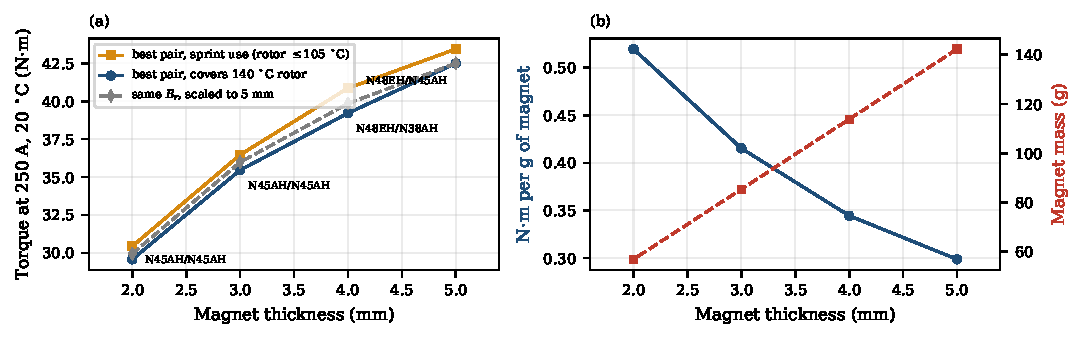
\includegraphics[width=\columnwidth]{thickness.pdf}
\caption{Magnet thickness. (a) Torque at \SI{250}{A} and \SI{20}{\celsius} for the best grade pair that covers a \SI{140}{\celsius} rotor, for the best pair for sprint use only, and for fixed $B_r$ (direct FEA, scaled to the 5-mm point). (b) Torque per gram of magnet and magnet mass.}
\label{fig:thick}
\end{figure}

\begin{table}[!t]
\caption{Magnet thickness: best grade pair and torque (ideal materials, \SI{250}{A})}\label{tab:thick}
\centering\footnotesize\setlength{\tabcolsep}{3.5pt}
\begin{tabular}{@{}cccccc@{}}
\toprule
$h_m$ & Pair (axial/side) & $T_{20}$ & $T_{100}$ & $T_\mathrm{mag,max}$ & Mass\\
(mm) & covers \SI{140}{\celsius} & (\Nm) & (\Nm) & nom./95\,\% (\si{\celsius}) & (g)\\
\midrule
5 & N48EH/N45AH & 42.5 & 38.8 & 145/137 & 142\\
4 & N48EH/N38AH & 39.2 & 35.9 & 142/136 & 114\\
3 & N45AH/N45AH & 35.5 & 32.3 & 149/142 & 85\\
2 & N45AH/N45AH & 29.6 & 26.9 & 143/137 & 57\\
\midrule
\multicolumn{6}{@{}l}{Sprint use only (rotor $\le$\SI{105}{\celsius}):}\\
5 & N50UH/N48EH & 43.4 & 39.6 & 117/-- & 142\\
4 & N50UH/N48EH & 40.9 & 37.2 & 111/-- & 114\\
3 & N48EH/N48EH & 36.5 & 33.2 & 121/-- & 85\\
2 & N48EH/N48EH & 30.4 & 27.6 & 115/-- & 57\\
\bottomrule
\end{tabular}
\end{table}


\Cref{fig:thick} and \cref{tab:thick} show the trade-off:
\begin{itemize}
\item \textbf{Torque falls by about \SI{3.5}{\Nm} per millimetre removed, and the fall accelerates below \SI{3}{mm}.} With the best pair for each thickness, \SI{4}{mm} gives \SI{-7.7}{\percent}, \SI{3}{mm} \SI{-16.6}{\percent} and \SI{2}{mm} \SI{-30}{\percent}.
\item \textbf{Torque per gram of magnet rises from 0.30 to \SI{0.52}{\Nm/g}.} This is why thin magnets are common where magnet cost or mass dominates.
\item \textbf{Thin magnets still need high-coercivity grades here.} In this machine the stator's reverse field at \SI{250}{A} is the design driver. Thinner magnets have a lower permeance coefficient, so they still need EH/AH grades to cover a hot rotor. The higher-$B_r$ grades do not become usable as the magnets get thinner.
\end{itemize}
Many published axial-flux motors with thin magnets are double-rotor or coreless, or run at lower electric loading, where this reverse field is weaker.

With the build and load factors of \cref{sec:realistic} (0.87) and the 6.6:1 reduction ($\eta=0.95$), the output torque at a \SI{100}{\celsius} rotor is about 213, 197, 177 and \SI{147}{\Nm} for 5, 4, 3 and \SI{2}{mm}. \SI{2}{mm} misses the \SI{180}{\Nm} target, and \SI{3}{mm} only meets it when the rotor is cool. \SI{4}{mm} is a reasonable trade if rotor inertia matters: it saves \SI{28}{g} and \SI{20}{\percent} of the magnet inertia for \SI{8}{\percent} torque. Otherwise \SI{5}{mm} remains the choice for maximum torque.


\section{Conclusion}
A full 3-D nonlinear magnetostatic FEA tool for axial-flux machines has been built on open-source finite-element libraries and documented. It solves the same physics as the magnetostatic solvers in commercial 3-D packages. Discretisation error is below \SI{1}{\percent}, and its load-dependent behaviour has been validated against a measured, published AFPM prototype. Compared with the multi-slice 2-D model, it reveals a 7--\SI{10}{\percent} torque reduction at peak current caused by end-region saturation. For the TREN-V4 motor with the v4b Halbach rotor it predicts \SI{41.5}{\Nm} at \SI{250}{A} with ideal materials. The realistic expectation for the built motor is about \SI{35}{\Nm} (33--\SI{38}{\Nm}). The main open uncertainties are the core stacking factor, magnet grade and temperature, and as-built gap, all of which a single locked-rotor test will resolve. In use the rotor stays below about \SI{105}{\celsius} except in continuous running at the stator limit, where it approaches \SI{140}{\celsius}. N48EH axial pieces with N45AH side pieces cover that case and give \SI{42.5}{\Nm} cold (ideal), about \SI{37}{\Nm} as built; 50-series SH and UH grades would demagnetise in this Halbach array. Thinner magnets cost about \SI{3.5}{\Nm} per millimetre; \SI{4}{mm} is a reasonable trade for lower inertia, while 3 and \SI{2}{mm} fall short of the output target when the rotor is warm.

\appendices
\section{Reproducing the Results}
The solver is released as openFLUX (\url{https://github.com/Qihaoguo30401/openFLUX}, Apache License 2.0). It requires Python~3.10+ and \texttt{pip install ngsolve}. The repository contains:
\begin{itemize}
\item \texttt{openflux/geometry.py}, \texttt{solver.py}, \texttt{materials.py}: the parametric axial-flux geometry, the nonlinear A-formulation solver with Arkkio torque, and the B-H data;
\item \texttt{examples/benchmark\_energies2020}: the published-prototype benchmark of Section~\ref{sec:verify}, with its raw results and post-processing.
\end{itemize}
The TREN-V4 geometry, the magnet-grade surrogate and Monte Carlo scripts and the rotor thermal model are not part of the public release. Each solve of the benchmark machine uses about \SI{6}{GB} of memory and 5--10~minutes on one core; run solves one at a time on a \SI{16}{GB} machine.

\FloatBarrier
\bibliographystyle{IEEEtran}
\bibliography{refs}

\end{document}
